\documentclass{beamer}
\usetheme{Singapore}
%\setbeamercolor{structure}{fg=red}
\usepackage{upgreek}
\usepackage{color}
%\def\magyarOptions{hyphenation=huhyphn}
%\usepackage{ae,aecompl}
%\usepackage[T1]{fontenc}
\usepackage[utf8]{inputenc}
%\usepackage[hungarian]{babel}
\usepackage{gensymb}
\usepackage{tikz}
\usepackage[framemethod=tikz]{mdframed}
\usepackage[version=3]{mhchem}


\normalfont
\title{Recent Advances in Potentiometric Scanning Electrochemical Microscopy}
\subtitle{Doctoral dissertation}
\author
{author:\\
András Kiss\\
\hfill \\
supervisor:\\
prof. Géza Nagy}

\institute
{
  %\inst{1}%
  Department of General and Physical Chemistry\\
  University of Pécs, Hungary\\
  \hfill \\

  
\includegraphics[width=0.14\textwidth]{pte_logo.eps}\\
  April 18, 2017
}

\date[]

\begin{document}
\frame{\titlepage}  


\begin{frame}
	\centering
	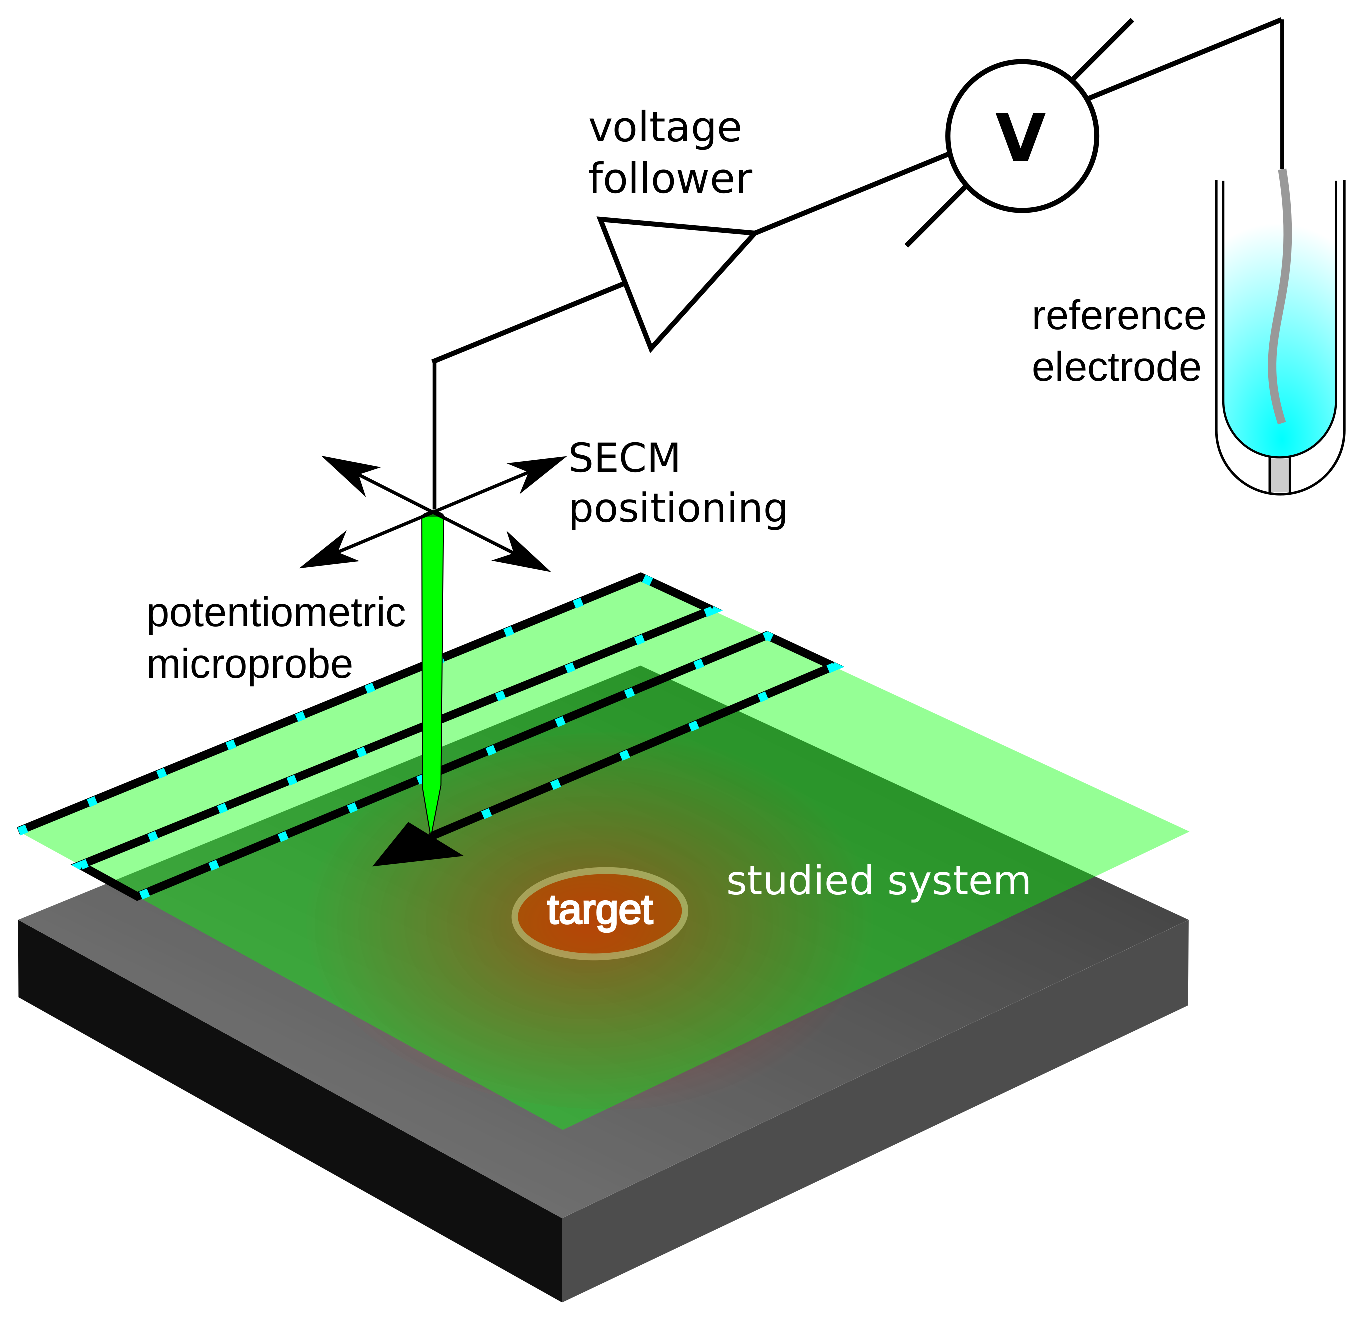
\includegraphics[width=0.6\textwidth]{secm.eps}
	\frametitle{Potentiometric Scanning Electrochemical Microscopy}
	\framesubtitle{A Scanning Probe Microscopic technique}

\end{frame}


\begin{frame}
\frametitle{Ion-selective micropipettes}
\framesubtitle{As SECM probes}
\begin{columns}[T] % align columns
\begin{column}{.48\textwidth}

\centering
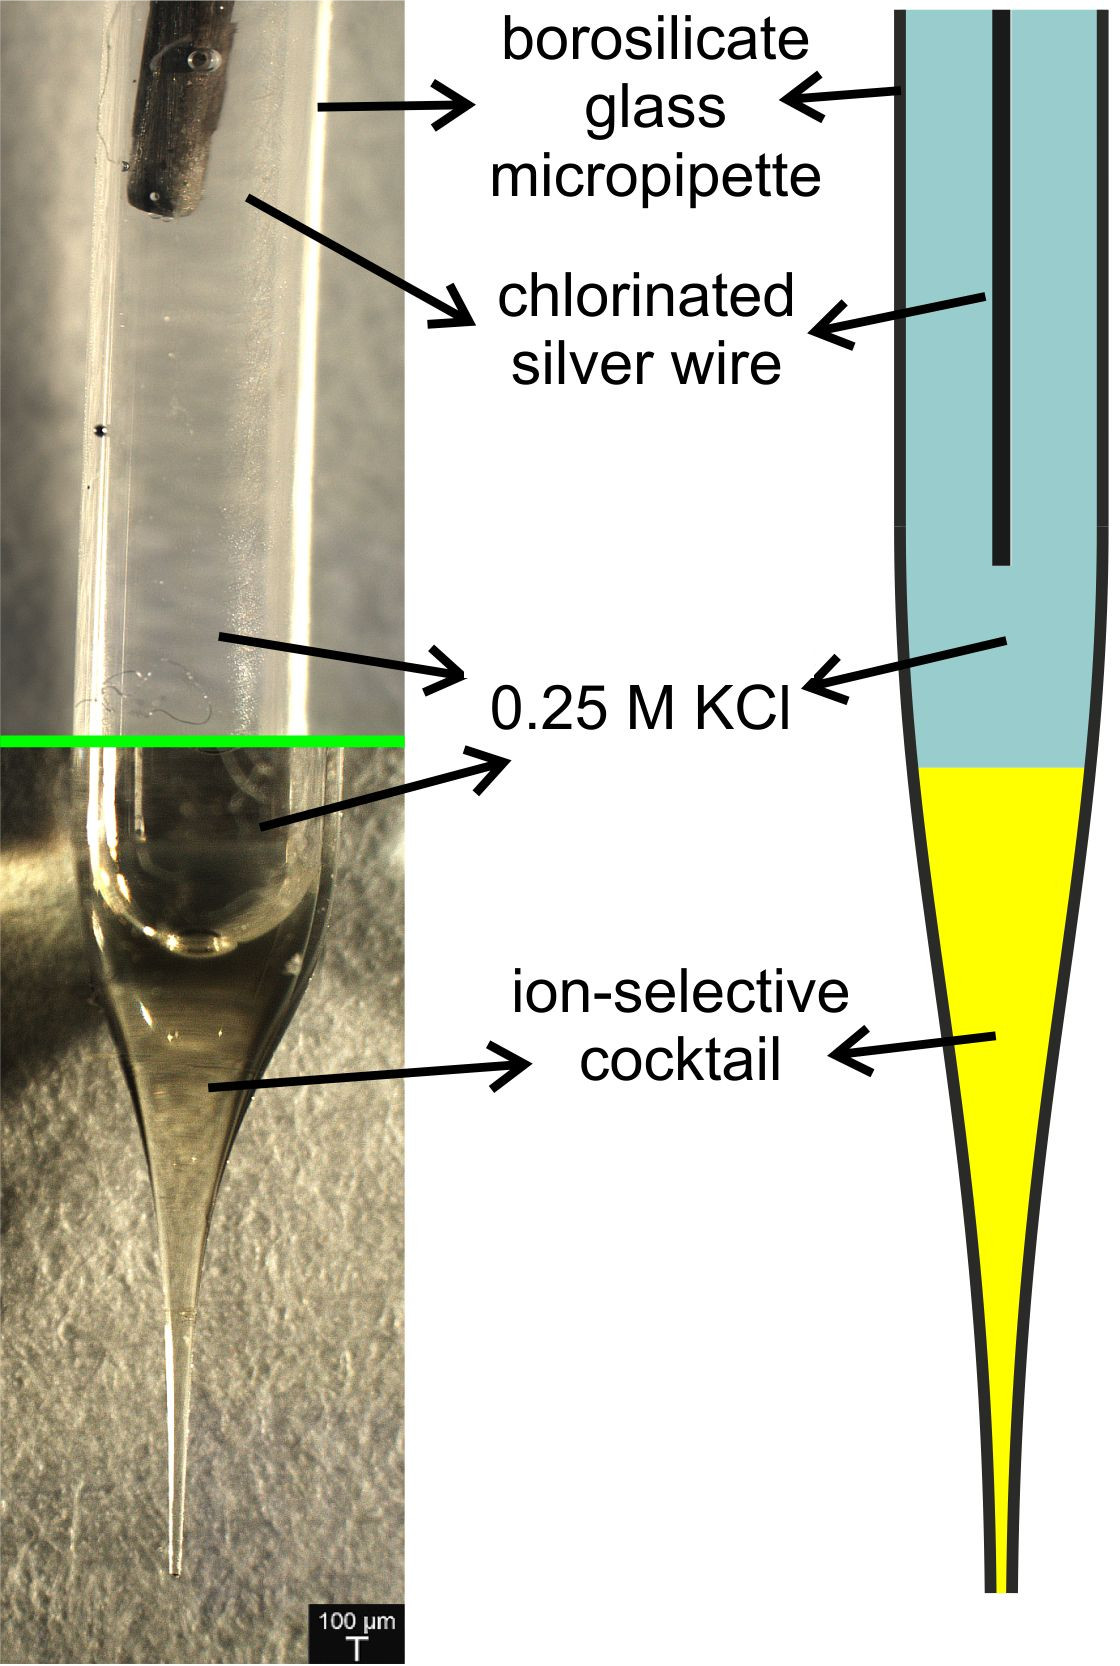
\includegraphics[width=0.9\textwidth]{liquid.jpg}
\end{column}%
\hfill%
\begin{column}{.48\textwidth}
%\color{blue}\rule{\linewidth}{4pt}
\centering

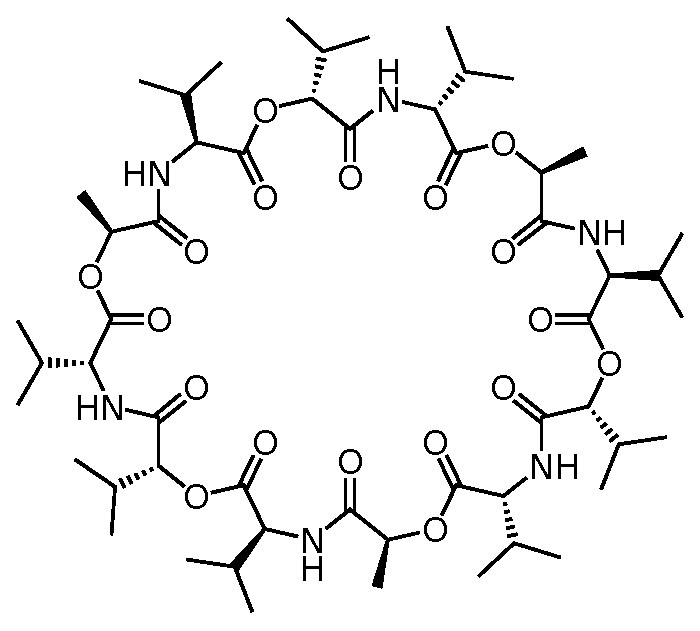
\includegraphics[width=0.8\textwidth]{Valinomycin.eps}

Valinomycin
\vfill

\footnotesize
\begin{equation*}
        E=E^\theta + \frac{RT}{z_iF} \ln \left [ a_i + \sum_{j} \left ( k_{ij}a_j^{z_i/z_j} \right ) \right ]
        \end{equation*}
\normalsize
Nikolsky--equation
\end{column}%
\end{columns}
\end{frame}

\begin{frame}
	\frametitle{The problem with potentiometric SECM} 
	\framesubtitle{Distortion at high scan rate}
	\centering
\quad\quad\quad\quad\quad\quad Slow \hfill Fast \quad\quad\quad\quad\quad\quad\quad

	\includegraphics[trim = 10mm 30mm 0mm 20mm, clip, width=0.4\textwidth, angle=-90]{real.eps}\hfill\includegraphics[trim = 10mm 30mm 0mm 20mm, clip, width=0.4\textwidth, angle=-90]{fastcomb_sim.eps}
\end{frame}

\begin{frame}
\frametitle{Why is the image distorted?}
\framesubtitle{Possible contributors to the lag}
\centering
\includegraphics[width=0.8\textwidth]{npp.eps}
\end{frame}

\begin{frame}
	\frametitle{Why is the image distorted?}
	\framesubtitle{The RC time constant} 
	\centering
	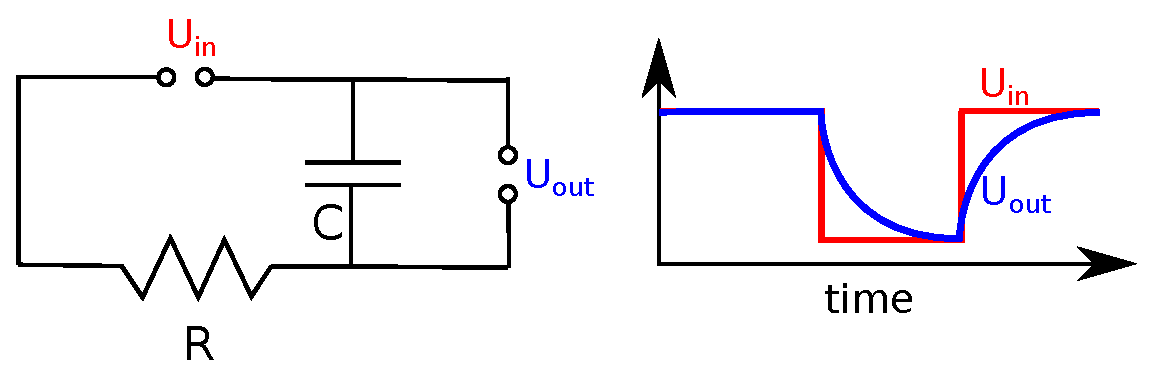
\includegraphics[width=1\textwidth]{RC.eps}
	\vfill
	The time that is required to charge \\ the capacitor by $\approx 63\%$ $(1-1/e)$.	
	\vfill
	$\tau = R \cdot C$
	
	$R = 5 $ G$\ohm$
	
	$C = 500 $ pF
	
	\textbf{\textcolor{white!100}{\colorbox{red!100}{$\tau = 2.5 $ s}}}

	%\includegraphics[width=0.6\textwidth, angle=-90]{meander_sim.eps}
\end{frame}

\begin{frame}
	\frametitle{Distortion of potentiometric imaging} 
	\framesubtitle{In the case of a linescan} 
	\centering
	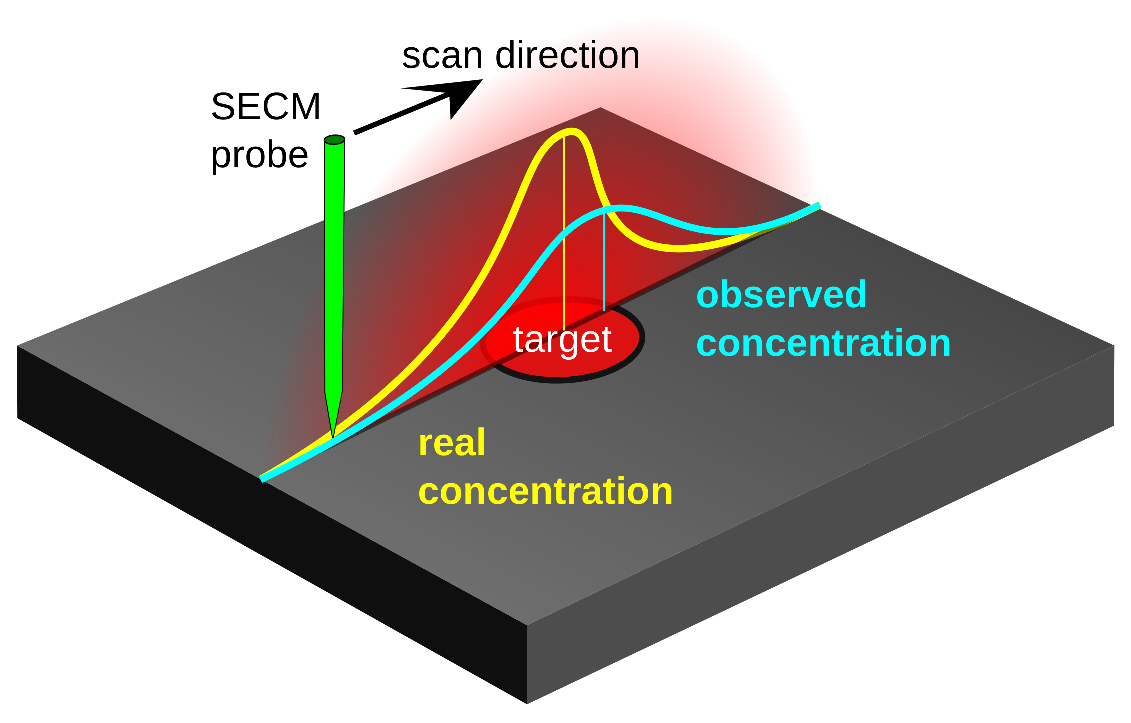
\includegraphics[width=0.8\textwidth]{distortion2.eps}
\end{frame}

\begin{frame}
	\frametitle{Why is it so important to complete the scan quickly?}
	\framesubtitle{Example: corrosion of a magnesium alloy}
	\includegraphics[width=1\textwidth]{timelapse.eps}\\
\centering
Corrosion of the AZ63 magnesium-aluminium-zinc alloy.
%Location of the anodic and cathodic spots change quickly. High-speed scanning is required to complete the scan before the studied system changes.
\end{frame} 

\begin{frame}
\frametitle{Trade-off triangle of potentiometric SECM}
\framesubtitle{Compromise between the three desired competing properties}
\begin{center}
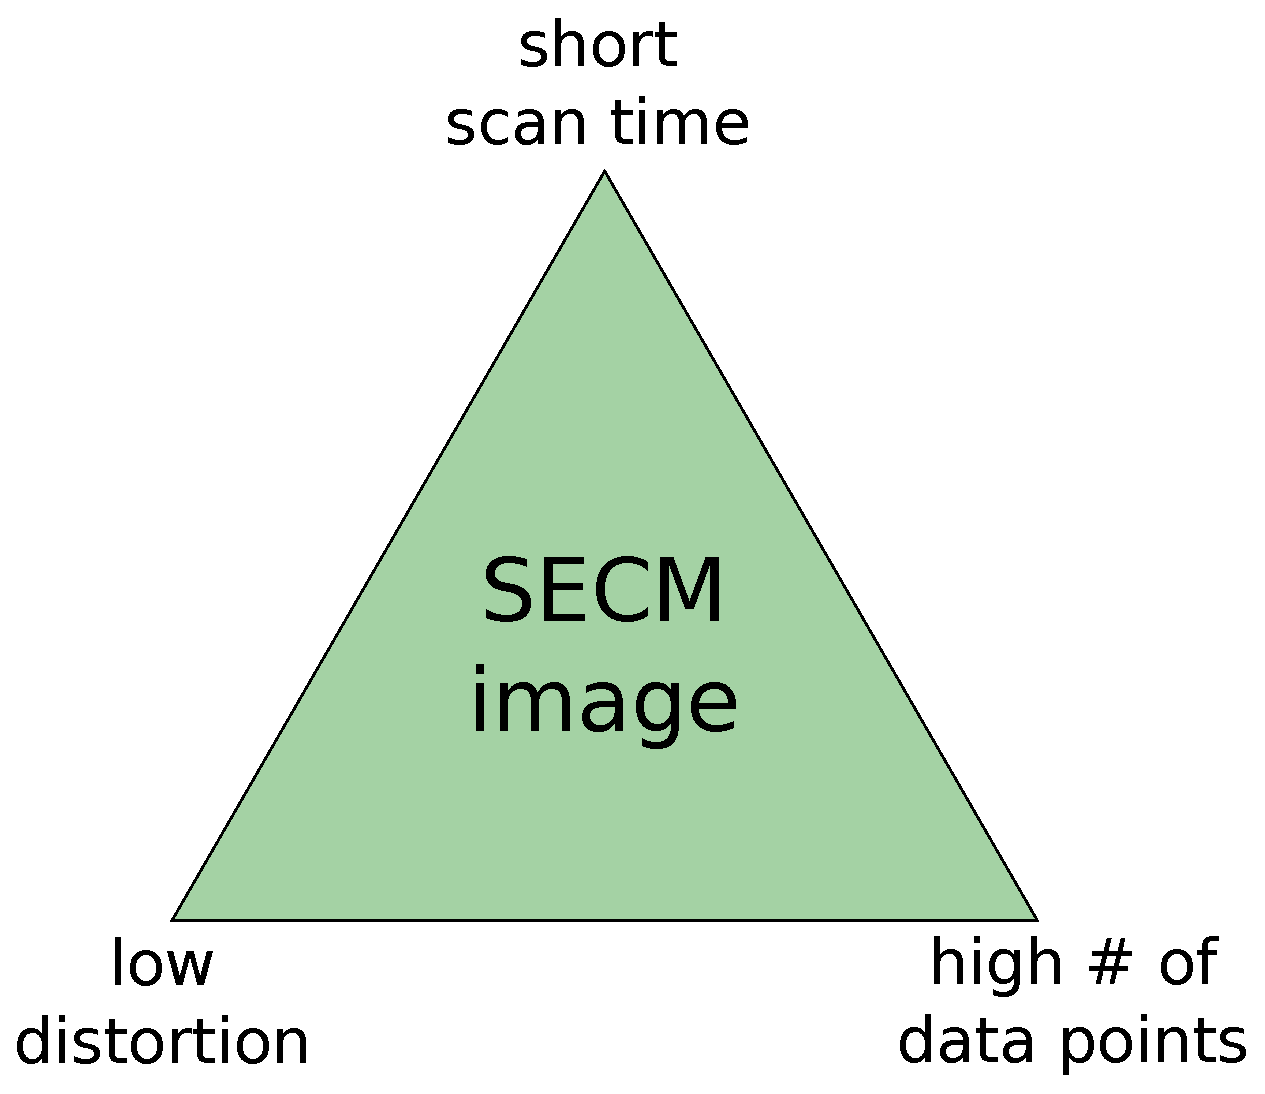
\includegraphics[width=0.5\textwidth]{trade-off.eps}
\end{center}
\end{frame}

\begin{frame}[plain]
\centering
Solution \#1:
Solid contact micropipettes as SECM probes.
\end{frame}

\begin{frame}
\frametitle{Liquid vs. solid contact micropipettes}
\framesubtitle{Comparison of construction}
\begin{center}
\quad\quad\quad\quad Liquid contact \hfill Solid contact \quad\quad\quad\quad

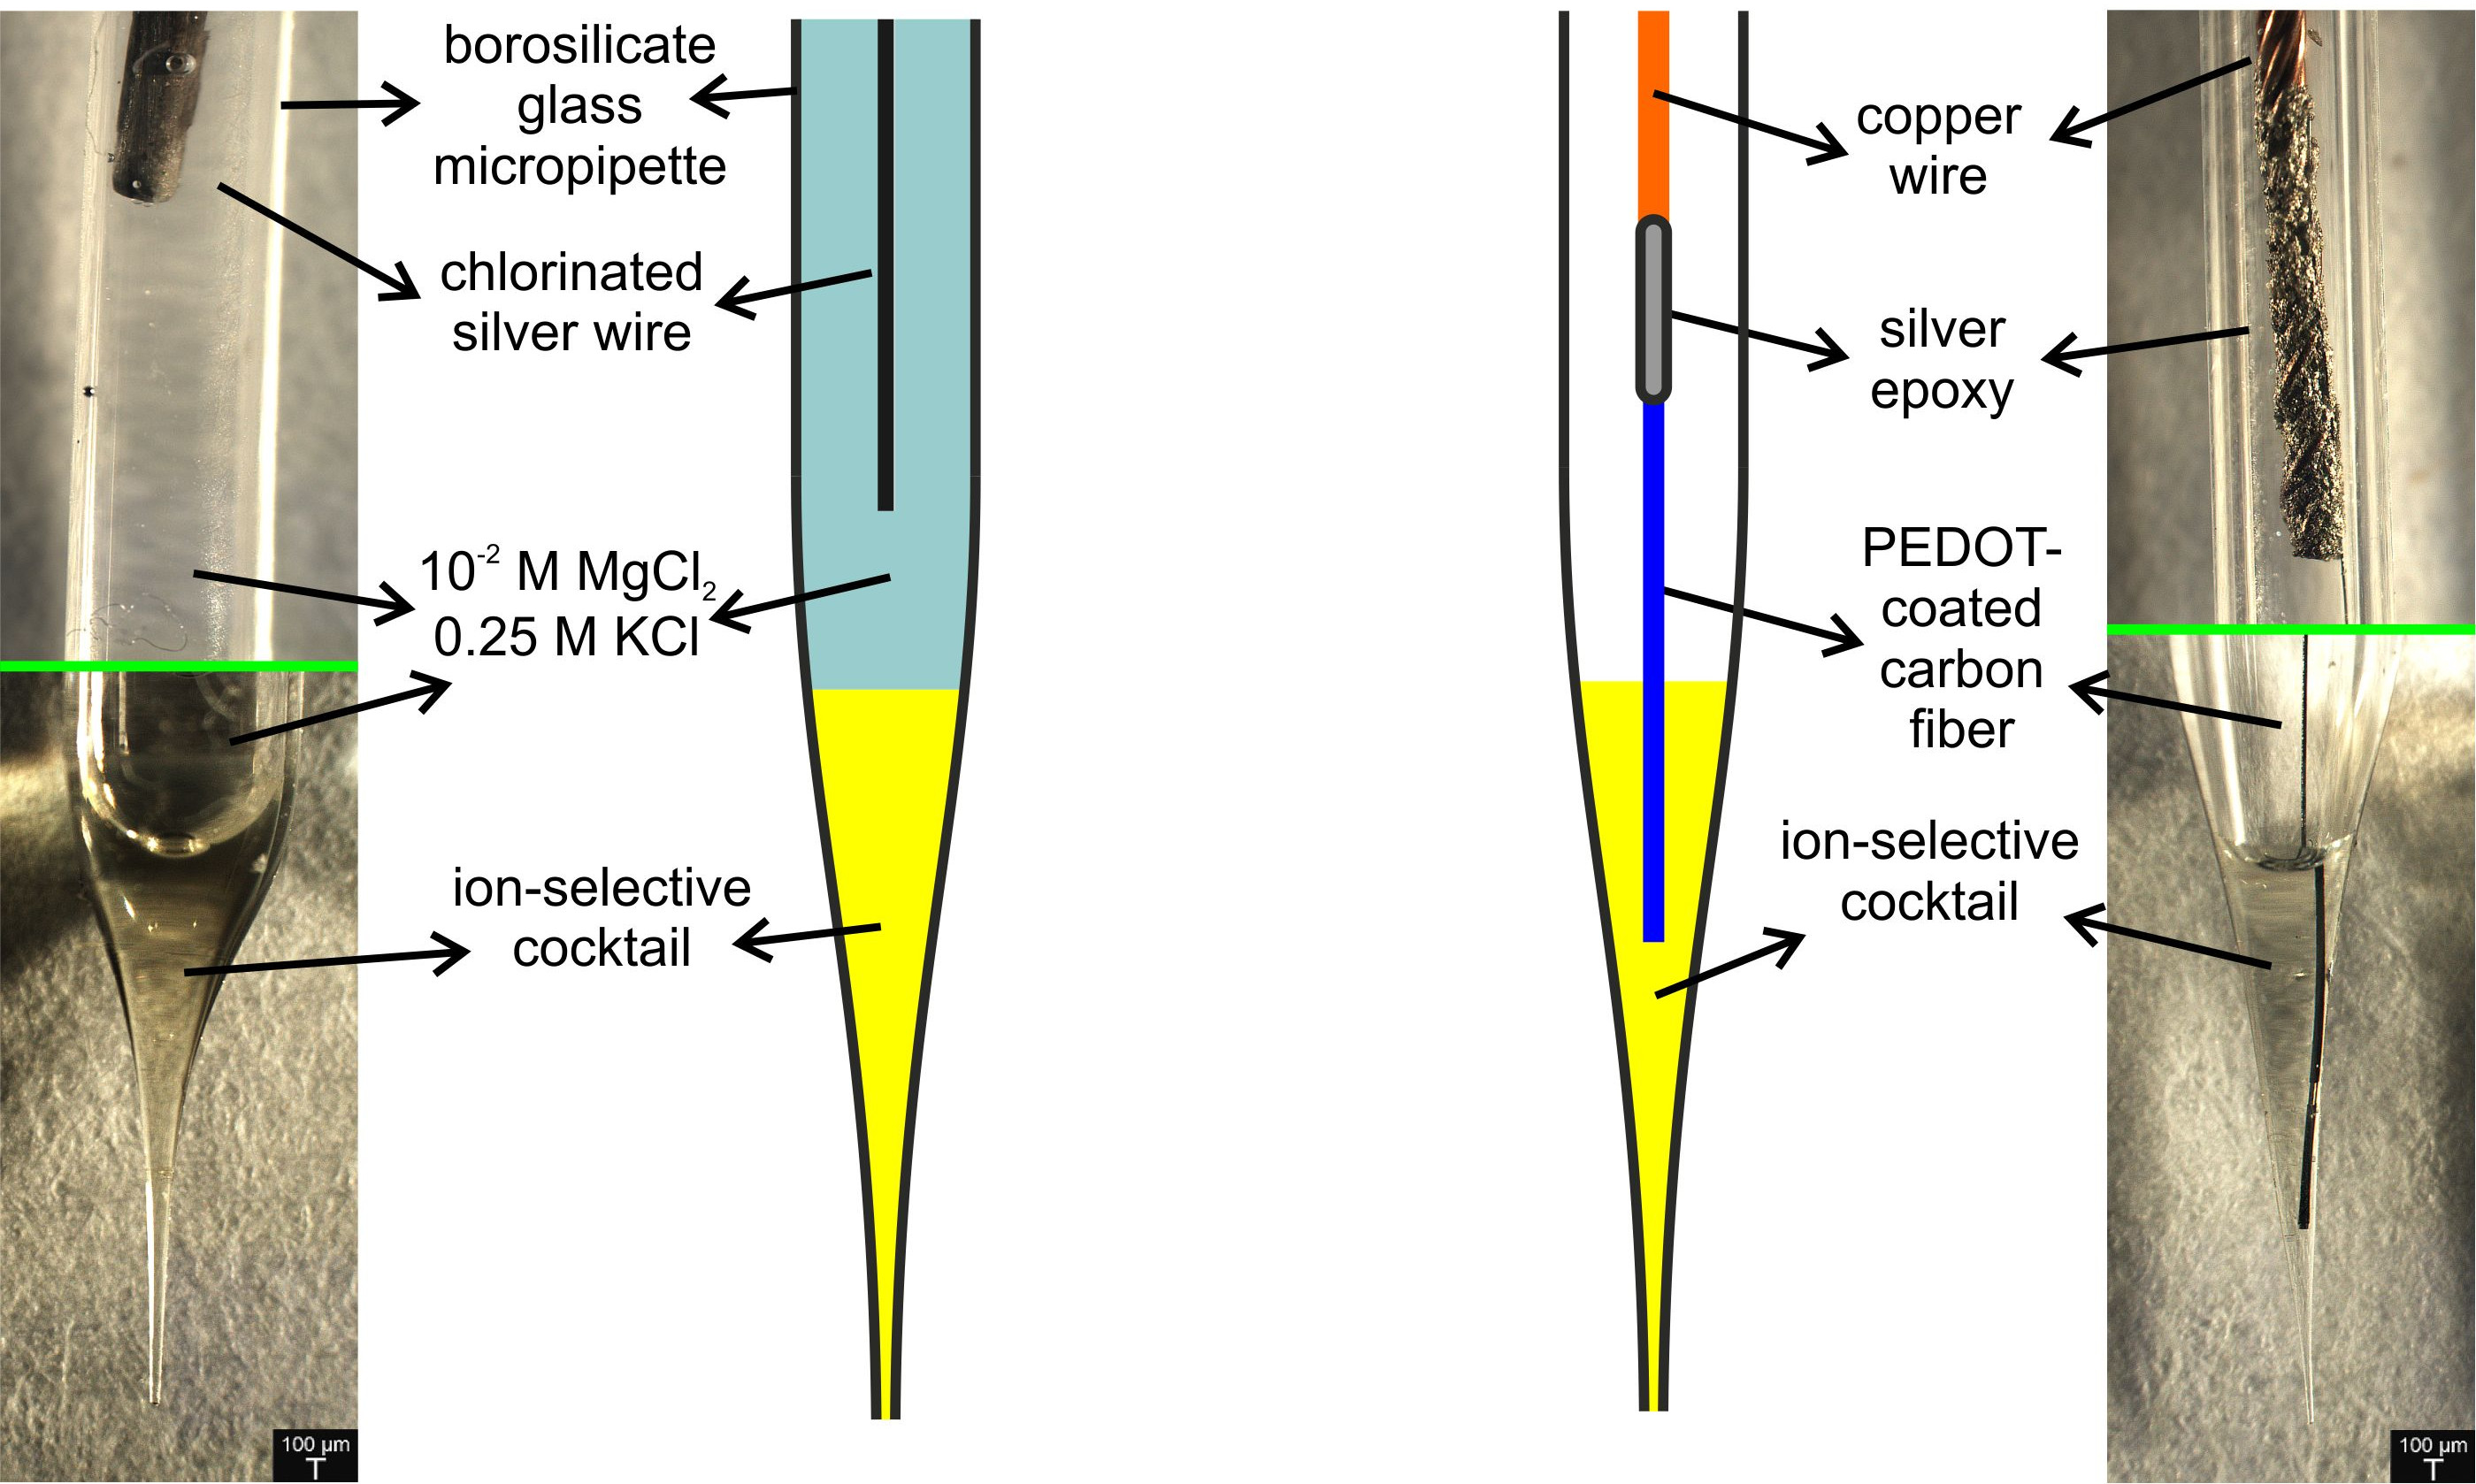
\includegraphics[width=0.9\textwidth]{liquid_solid.jpg}
\end{center}
\end{frame}

\begin{frame}
\frametitle{Comparison of the electrodes' resistance}
\framesubtitle{Voltage divider method and result}
\begin{center}
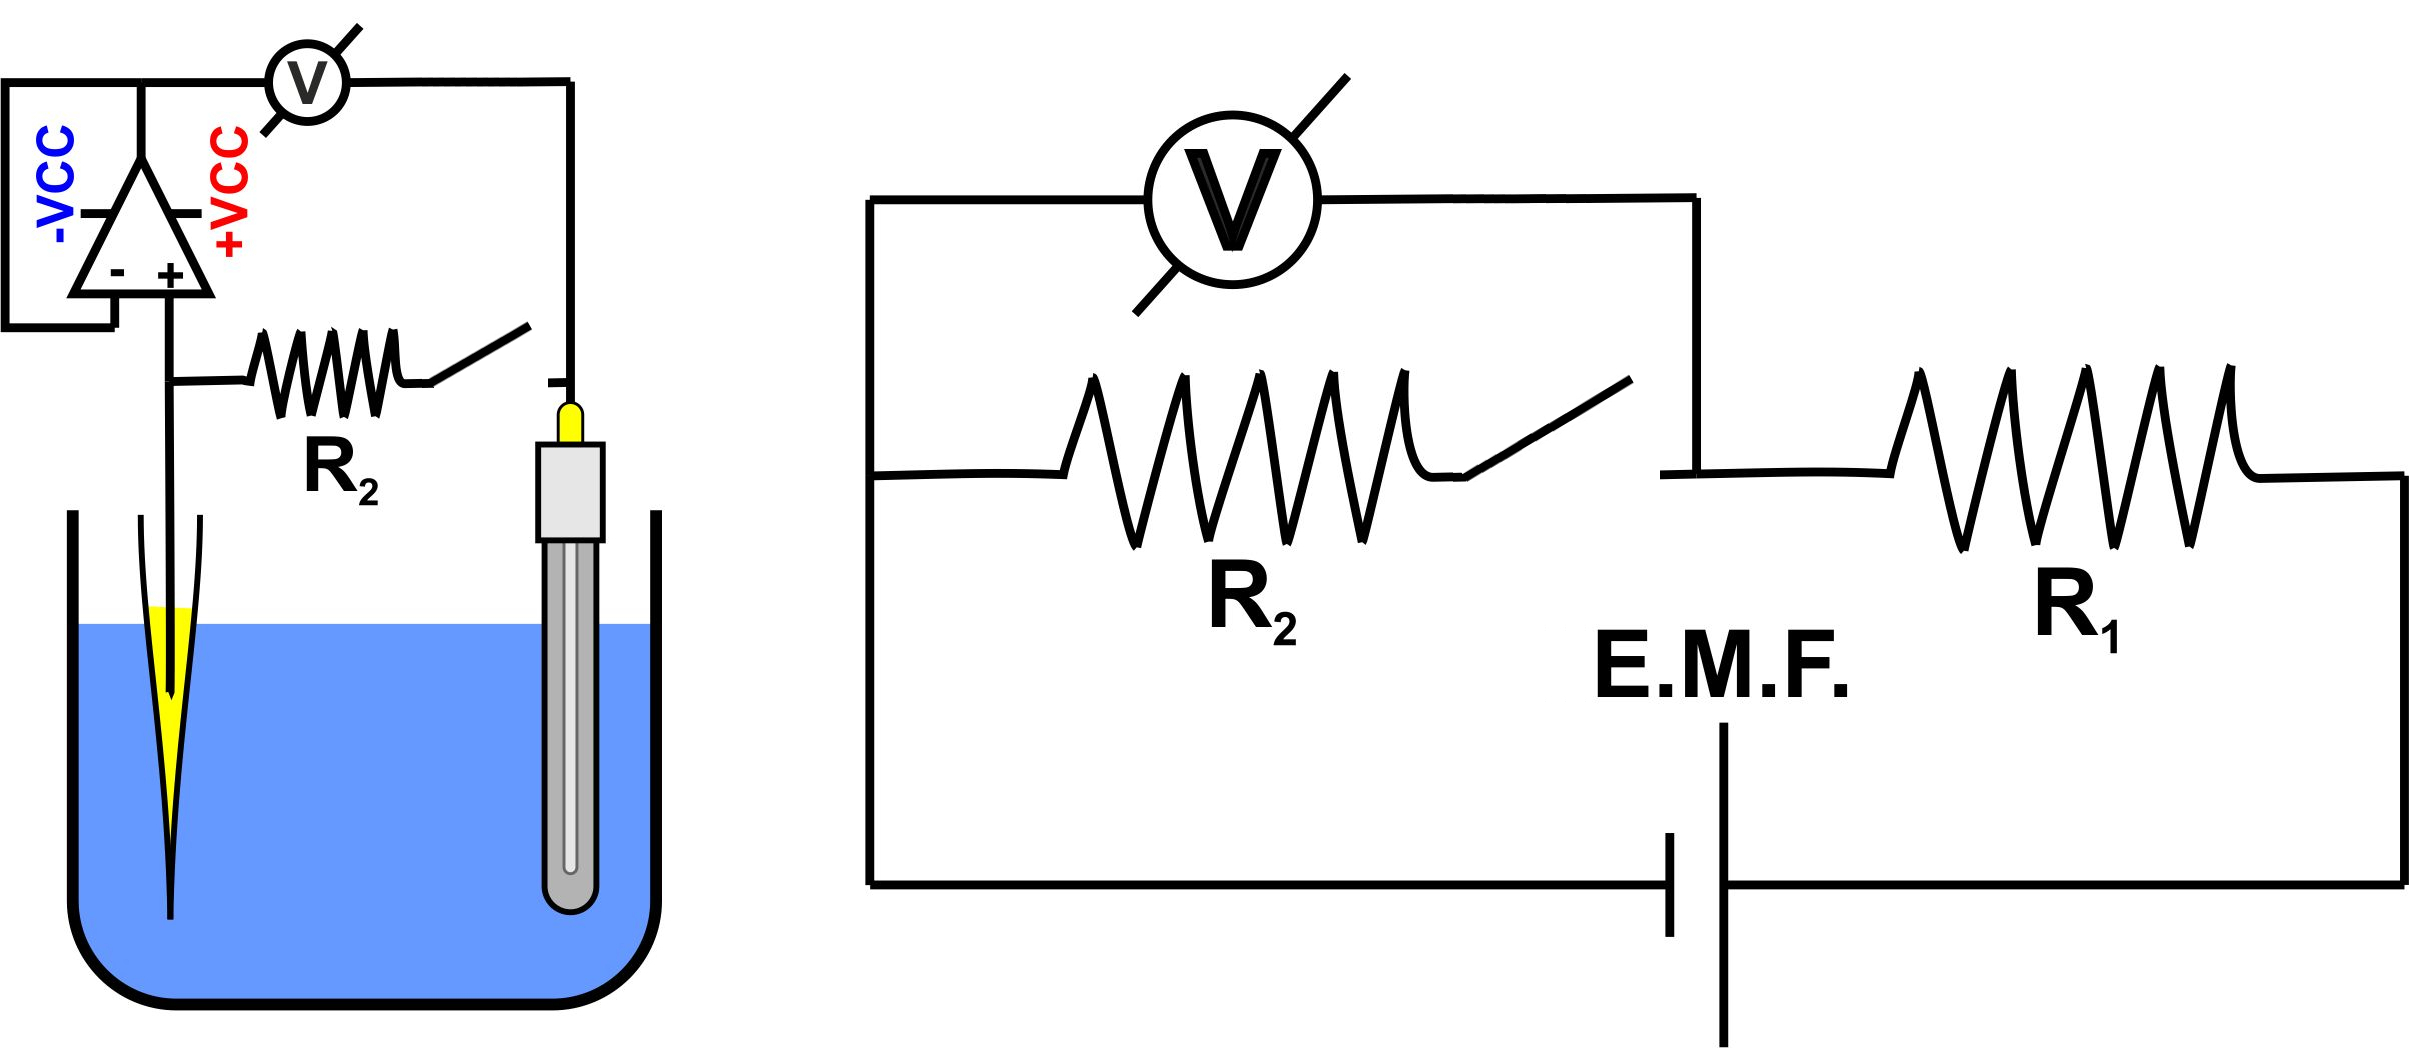
\includegraphics[width=0.7\textwidth]{divider_switch.jpg}
\vfill
\begin{table}
                \centering
                \begin{tabular}{r c}
                        %\hline
                        Type & R$_{ISME}$ / G$\ohm$ \\
			\cline{1-2}
			Liquid contact & \textbf{\textcolor{white!100}{\colorbox{red!100}{4.80}}} \\
                        Solid contact &  \textbf{\textcolor{black!100}{\colorbox{green!100}{0.56}}} \\

                \end{tabular}
\end{table}
\end{center}
\end{frame}

\begin{frame}
\frametitle{Comparison of the electrodes' performance}
\framesubtitle{Experimental setup}
\begin{center}
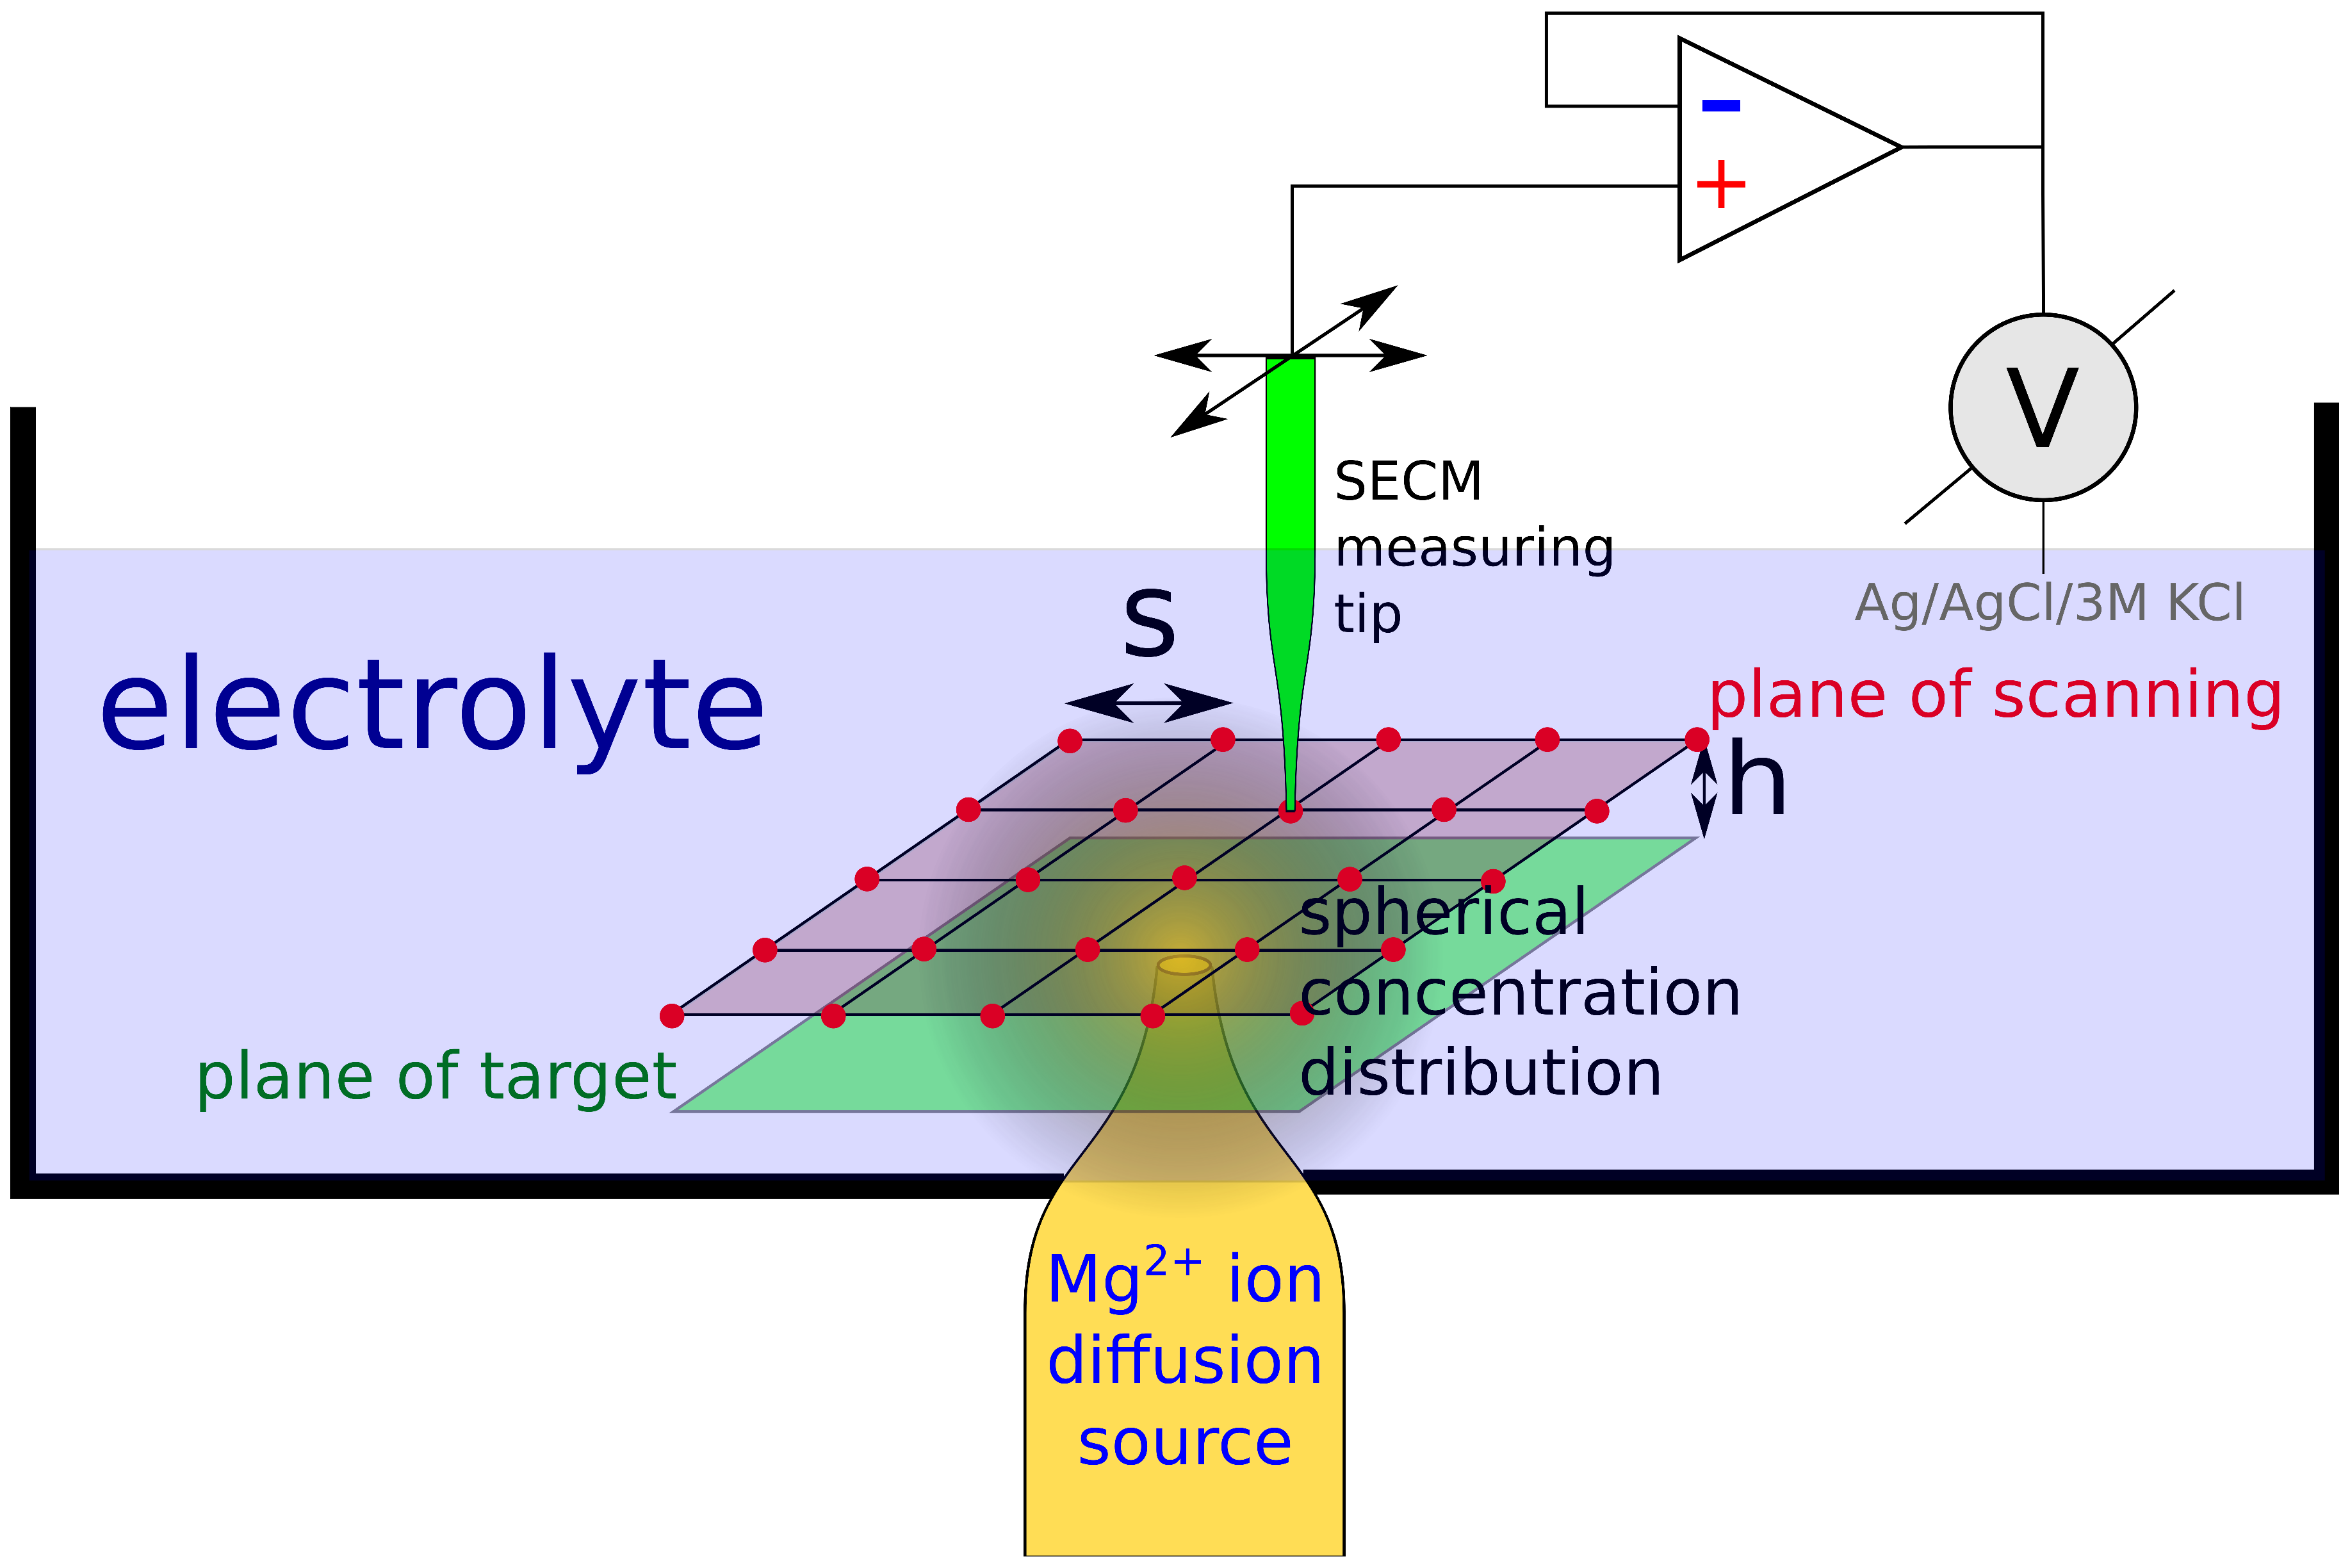
\includegraphics[width=0.9\textwidth]{setup.eps}
\end{center}
\end{frame}

\begin{frame}
	\frametitle{Comparison of the electrodes' performance} 
	\framesubtitle{Results}
	\centering
	\quad\quad\quad\quad Liquid contact \hfill Solid contact \quad\quad\quad\quad\quad

	\includegraphics[trim = 10mm 30mm 0mm 20mm, clip, width=0.4\textwidth, angle=-90]{liquid_Mg.eps}\hfill\includegraphics[trim = 10mm 30mm 0mm 20mm, clip, width=0.4\textwidth, angle=-90]{solid_Mg.eps}
\end{frame}

\begin{frame}
\frametitle{Application in corrosion science: galvanic corrosion of Mg}
\framesubtitle{Experimental setup}
\begin{center}
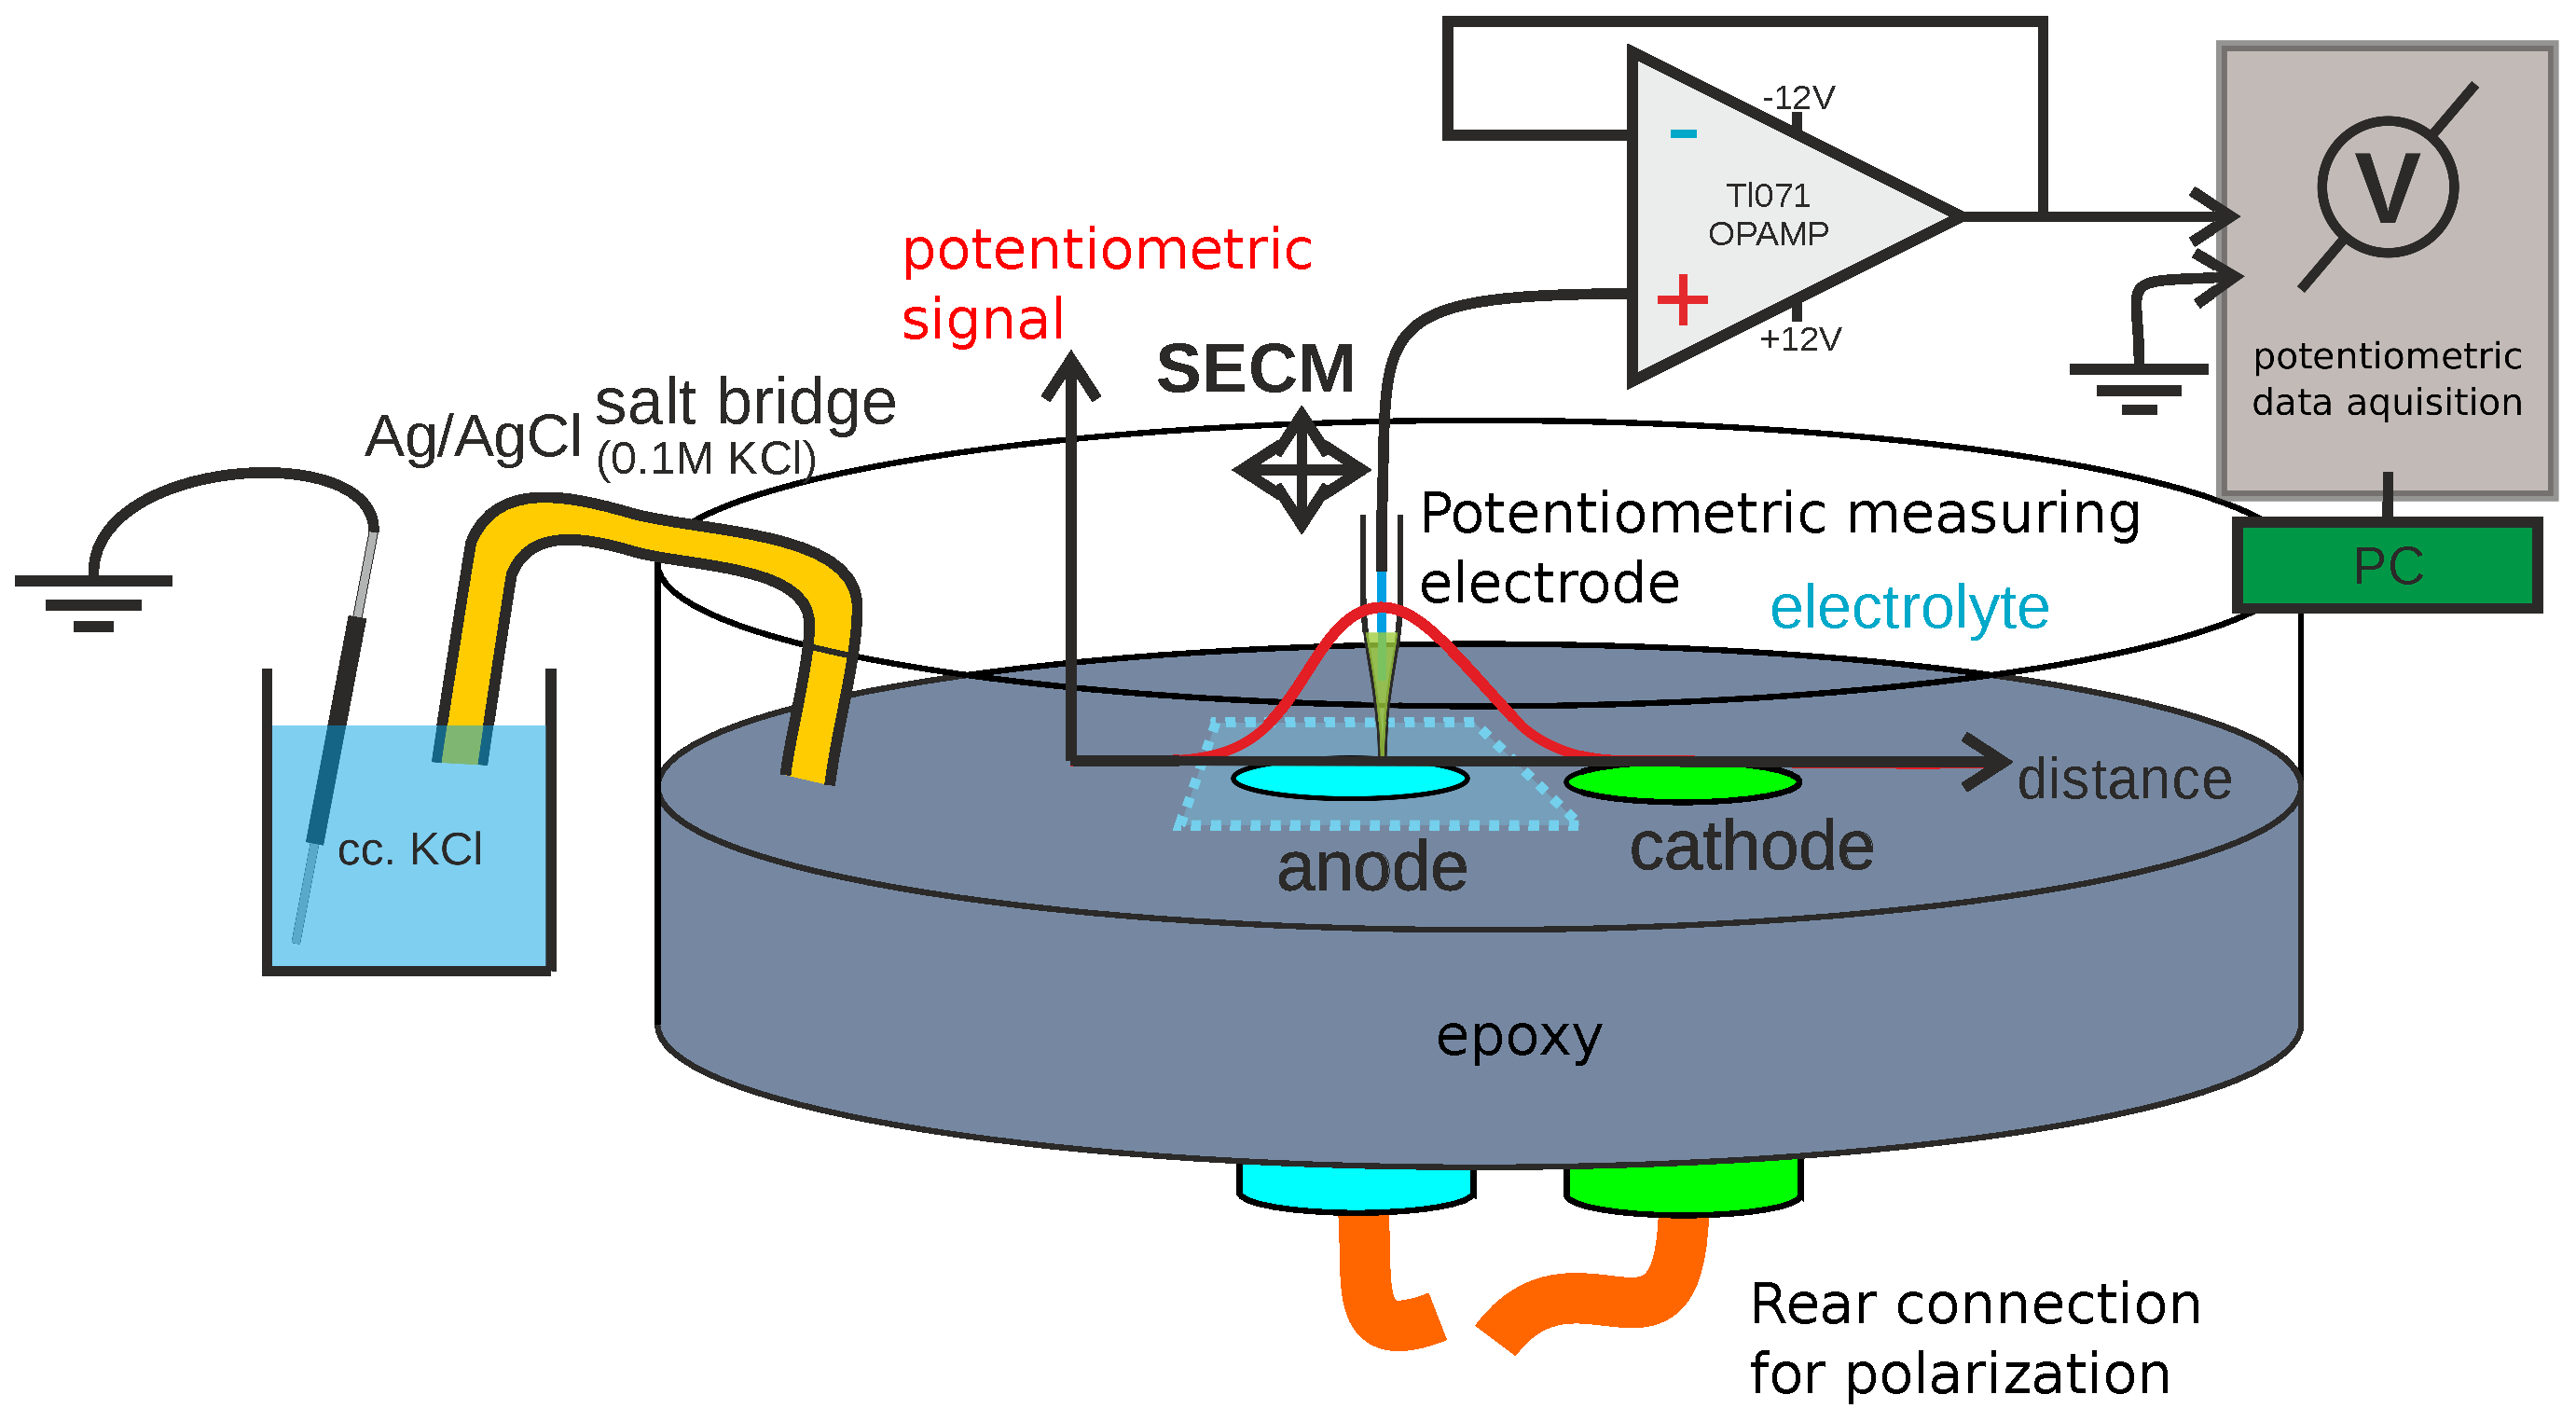
\includegraphics[width=0.9\textwidth]{model.eps}
\end{center}
\end{frame}

\begin{frame}
	\frametitle{Application in corrosion science: galvanic corrosion of Mg} 
	\framesubtitle{Results}
	\centering
	\quad\quad\quad\quad Liquid contact \hfill Solid contact \quad\quad\quad\quad\quad

	\includegraphics[trim = 10mm 30mm 0mm 20mm, clip, width=0.4\textwidth, angle=-90]{liquid_coupled.eps}\includegraphics[trim = 10mm 30mm 0mm 20mm, clip, width=0.4\textwidth, angle=-90]{solid_coupled.eps}
\end{frame}



\begin{frame} [plain]
\centering
Solution \#2:
Optimizing scanning patterns and algorithms.
\end{frame}

\begin{frame}
	\frametitle{New SECM scanning patterns based on the polar-coordinate system}
	\centering	
	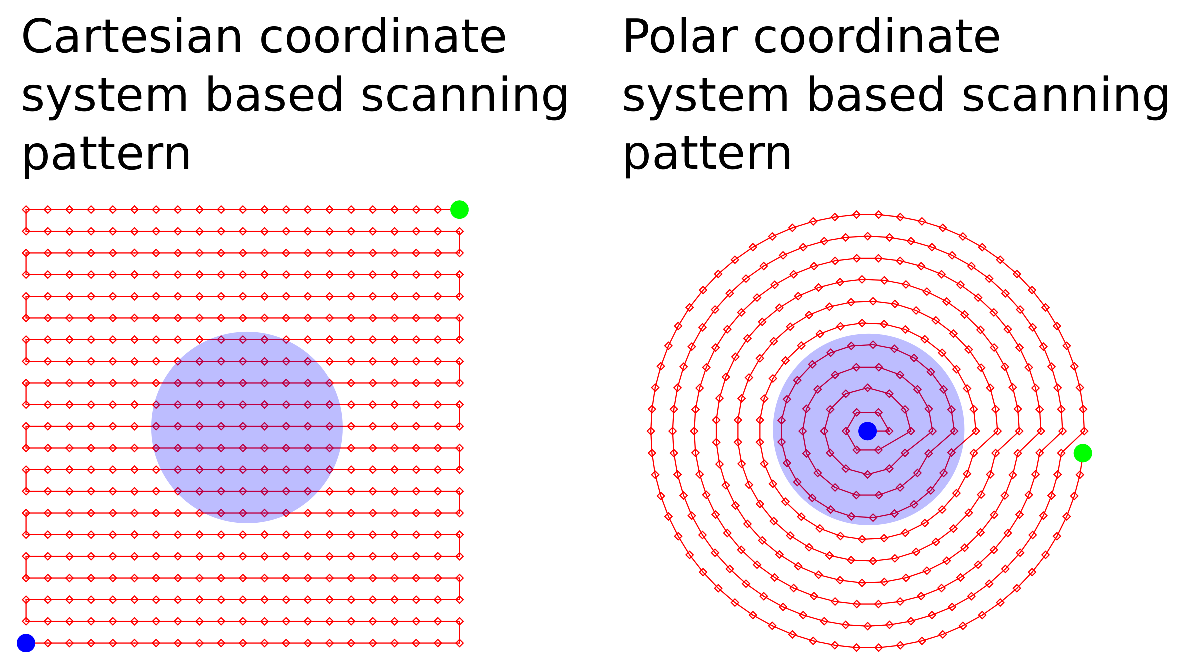
\includegraphics[width=0.7\textwidth]{cartesian_vs_polar.eps}
	
	\vfill
\end{frame}

\begin{frame}
	\frametitle{Simulated SECM scans}	
	\framesubtitle{Using the Cartesian and the polar coordinate system based algorithms}
	\centering
	\quad\quad\quad\quad\quad\quad Cartesian \hfill polar \quad\quad\quad\quad\quad\quad\quad\quad

	\includegraphics[width=0.3\textwidth, angle=-90]{meander_sim.eps}\includegraphics[width=0.3\textwidth, angle=-90]{arc_sim.eps}
	\vfill
\end{frame}


\begin{frame}
	\frametitle{Comparison of the simulated scans}
%Parameters of the simulations:\\
%\begin{itemize}
%\item 2000 $\upmu$m $\times$ 2000 $\upmu$m scan area,
%\item 100 $\upmu$m $\times$ 100 $\upmu$m resolution,
%\item 1 s for each data aquisition point,
%\item 500 $\upmu$m/s probe positioning speed.
%\end{itemize}

%\vfill
\begin{table}
		\label{table:comp}
		\centering
		\begin{tabular}{r c c c}
			Algorithm & n & time (s) & mean squared error \\
			\hline
			Meander & 441 & 440 & \textcolor{white!100}{\colorbox{red!100}{$2.75\times 10^{-2}$}} \\
			Fast comb& 441 & 520  & \colorbox{white}{$2.07\times 10^{-2}$} \\
			Comb & 441 & 881 & \colorbox{white}{$2.75\times 10^{-2}$} \\
			Web & 110 & 109 & \colorbox{white}{$9.63\times 10^{-3}$} \\
			Arc & 341 & 340 & \colorbox{green!100}{$2.95\times 10^{-3}$} \\
		\end{tabular}
\end{table}
\end{frame}

%\begin{frame}
%\frametitle{Confirmation with experimental SECM scans}
%\framesubtitle{Antimony microelectrode as pH sensor}
%\centering
%\begin{equation*}
%    \ce{2Sb + 3H_2O <=> Sb_2O_3 + 6H^+ + 6e^-}
%\end{equation*}
%\includegraphics[width=0.7\textwidth]{antimony.eps}
%\end{frame} 


\begin{frame}
	\centering
	\frametitle{Confirmation with experimental SECM scans}
	\framesubtitle{Recorded using the antimony microelectrode}
	\quad\quad\quad\quad\quad 440 seconds \hfill 340 seconds \quad\quad\quad\quad\quad\quad


	\includegraphics[width=0.3\textwidth, angle=-90]{meander.eps}\includegraphics[width=0.3\textwidth, angle=-90]{arc.eps}\\
	\vfill
	Scans are completed almost 2 times faster,\\ images have almost 10 times less distortion.
\end{frame}

\begin{frame}[plain]
\centering
Solution \#3: Signal processing.
\end{frame}

\begin{frame}
\frametitle{The convolution function of the distortion}
\centering	
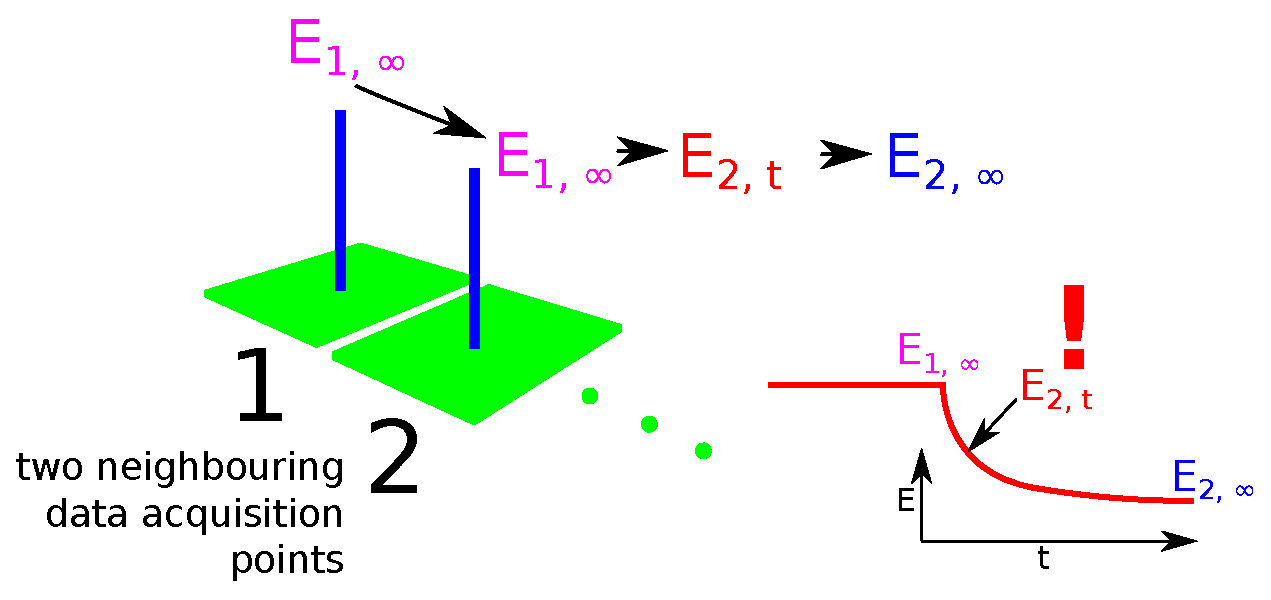
\includegraphics[width=1\textwidth]{t.eps}\\
\vfill
$E_{cell}(t) = E_{cell}(\infty) + [E_{cell}(0) - E_{cell}(\infty)]e^{-t/\tau}$\\
\vfill
%$E_{cell}(\infty)	= \frac {\displaystyle [E_{cell}(t) - E_{cell}(0)]e^{-t/RC}}	{\displaystyle 1 - e^{-t/RC}}$
\end{frame}

\begin{frame}
\frametitle{Convolution and deconvolution}
\centering
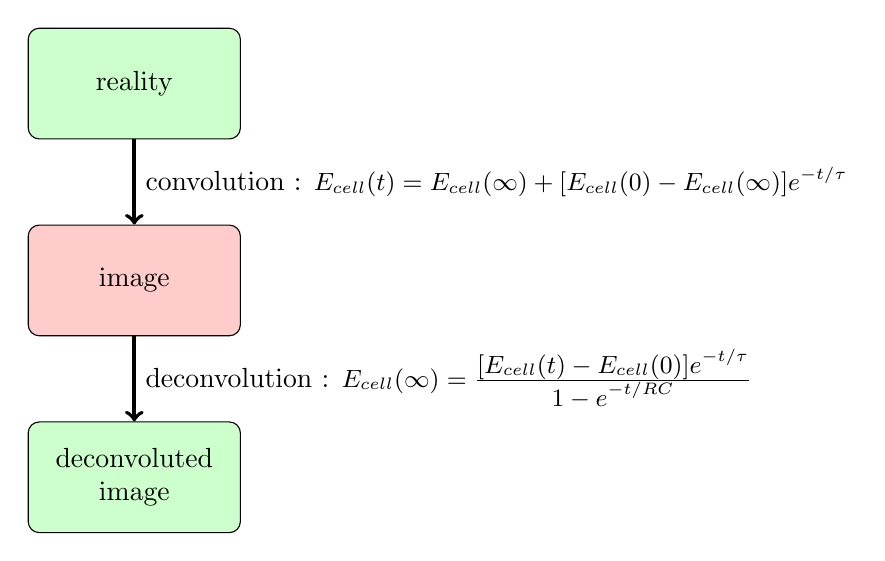
\begin{tikzpicture}[node distance = 2.5cm, auto]
\node [rectangle, draw, fill=green!20,text width=7em, text centered, rounded corners, minimum height=4em] (reality) {reality};
\node [rectangle, below of=reality, draw, fill=red!20,text width=7em, text centered, rounded corners, minimum height=4em] (measurement) {image};
\node [rectangle, below of=measurement, draw, fill=green!20,text width=7em, text centered, rounded corners, minimum height=4em] (image) {deconvoluted\\ image};

\draw [line width=0.5mm, ->] (reality) -- (measurement) node [pos=.5, right] (TextNode) {convolution : \small $E_{cell}(t) = E_{cell}(\infty) + [E_{cell}(0) - E_{cell}(\infty)]e^{-t/\tau}$};
\draw [line width=0.5mm, ->] (measurement) -- (image) node [pos=.5, right] (TextNode) {deconvolution : \small $E_{cell}(\infty)      = \frac {\displaystyle [E_{cell}(t) - E_{cell}(0)]e^{-t/\tau}}    {\displaystyle 1 - e^{-t/RC}}$};


\end{tikzpicture}
\end{frame}


\begin{frame}
	\frametitle{Deconvolution of potentiometric SECM images}
	\framesubtitle{Recorded using the antimony microelectrode following the meander algorithm}
\centering

\def\s{0.15}

\begin{columns}[T] % align columns

\begin{column}{.2\textwidth}
\begin{minipage}[c][0.75\textheight][c]{\linewidth}
\centering
%raw\\
%images
\end{minipage}
\end{column}%
\hfill%
\begin{column}{.2\textwidth}
\centering
\includegraphics[trim = 10mm 30mm 0mm 10mm, clip, width=0.8\textwidth, angle=-90]{13121313.eps}\\
\includegraphics[trim = 10mm 30mm 0mm 10mm, clip, width=0.8\textwidth, angle=-90]{13121314.eps}\\
\includegraphics[trim = 10mm 30mm 0mm 10mm, clip, width=0.8\textwidth, angle=-90]{13121315.eps}\\
\includegraphics[trim = 10mm 30mm 0mm 10mm, clip, width=0.8\textwidth, angle=-90]{13121316.eps}\\
\end{column}%
\begin{column}{.2\textwidth}
\begin{minipage}[c][0.7\textheight][c]{\linewidth}
\centering
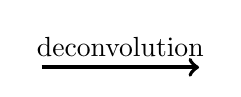
\begin{tikzpicture}
\draw [line width=0.5mm,->] (0,0) -- (2,0) node [pos=.5, above] (TextNode) {deconvolution};
\end{tikzpicture}
\end{minipage}
\end{column}%
\begin{column}{.2\textwidth}
\centering
\includegraphics[trim = 10mm 30mm 0mm 10mm, clip, width=0.8\textwidth, angle=-90]{13121313_deconvoluted.eps}\\
\includegraphics[trim = 10mm 30mm 0mm 10mm, clip, width=0.8\textwidth, angle=-90]{13121314_deconvoluted.eps}\\
\includegraphics[trim = 10mm 30mm 0mm 10mm, clip, width=0.8\textwidth, angle=-90]{13121315_deconvoluted.eps}\\
\includegraphics[trim = 10mm 30mm 0mm 10mm, clip, width=0.8\textwidth, angle=-90]{13121316_deconvoluted.eps}\\
\end{column}%
\begin{column}{.2\textwidth}
\begin{minipage}[c][0.75\textheight][c]{\linewidth}
\centering
%deconvoluted\\
%images
\end{minipage}
\end{column}%
\end{columns}
\end{frame}

\begin{frame}
\begin{center}
\frametitle{Deconvolution of potentiometric SECM images}
\framesubtitle{Recorded using the magnesium ISME following the meander algorithm}
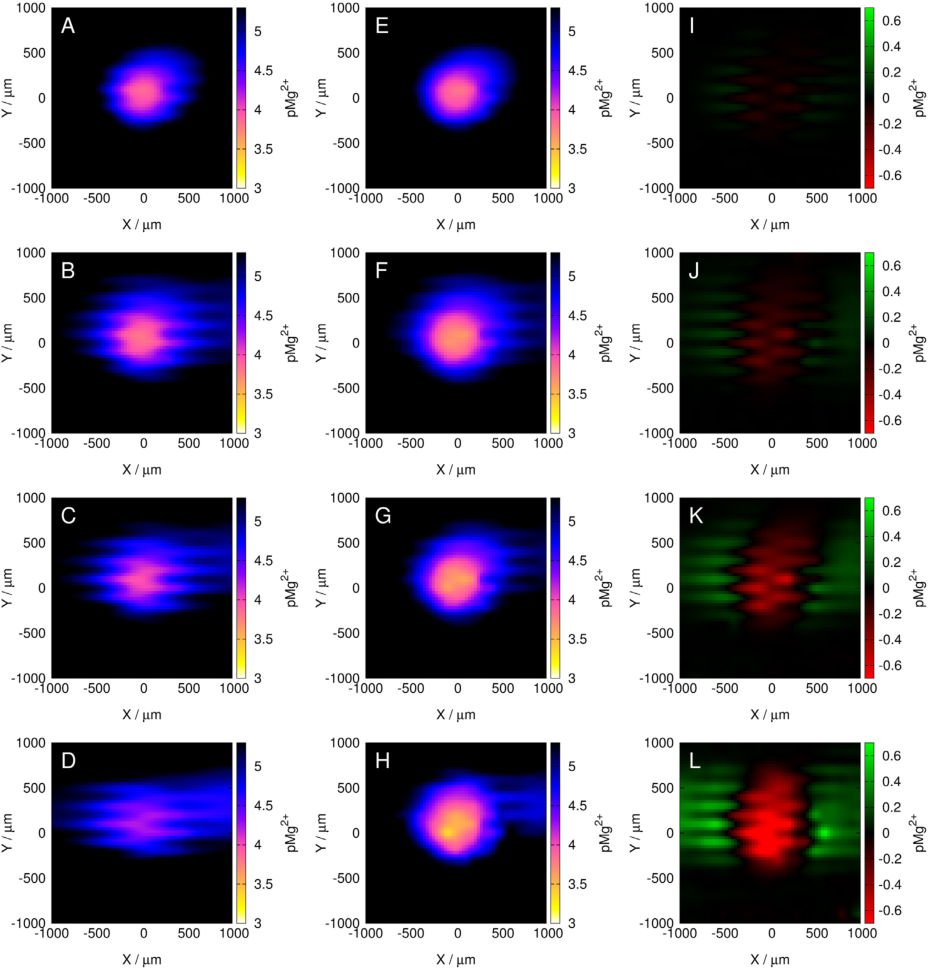
\includegraphics[width=0.6\textwidth]{mg_2d.pdf}
\end{center}
\end{frame}

\begin{frame}
\frametitle{Practical example: corroding carbon steel sample}
\framesubtitle{Scanned with an antimony microelectrode}
\begin{figure}
\centering
%top left bottom right
\includegraphics[trim = 10mm 30mm 0mm 10mm, clip, width=0.3\textwidth, angle=-90]{16012906.eps}\includegraphics[trim = 10mm 30mm 0mm 10mm, clip, width=0.3\textwidth, angle=-90]{16012906_deconvoluted.eps}

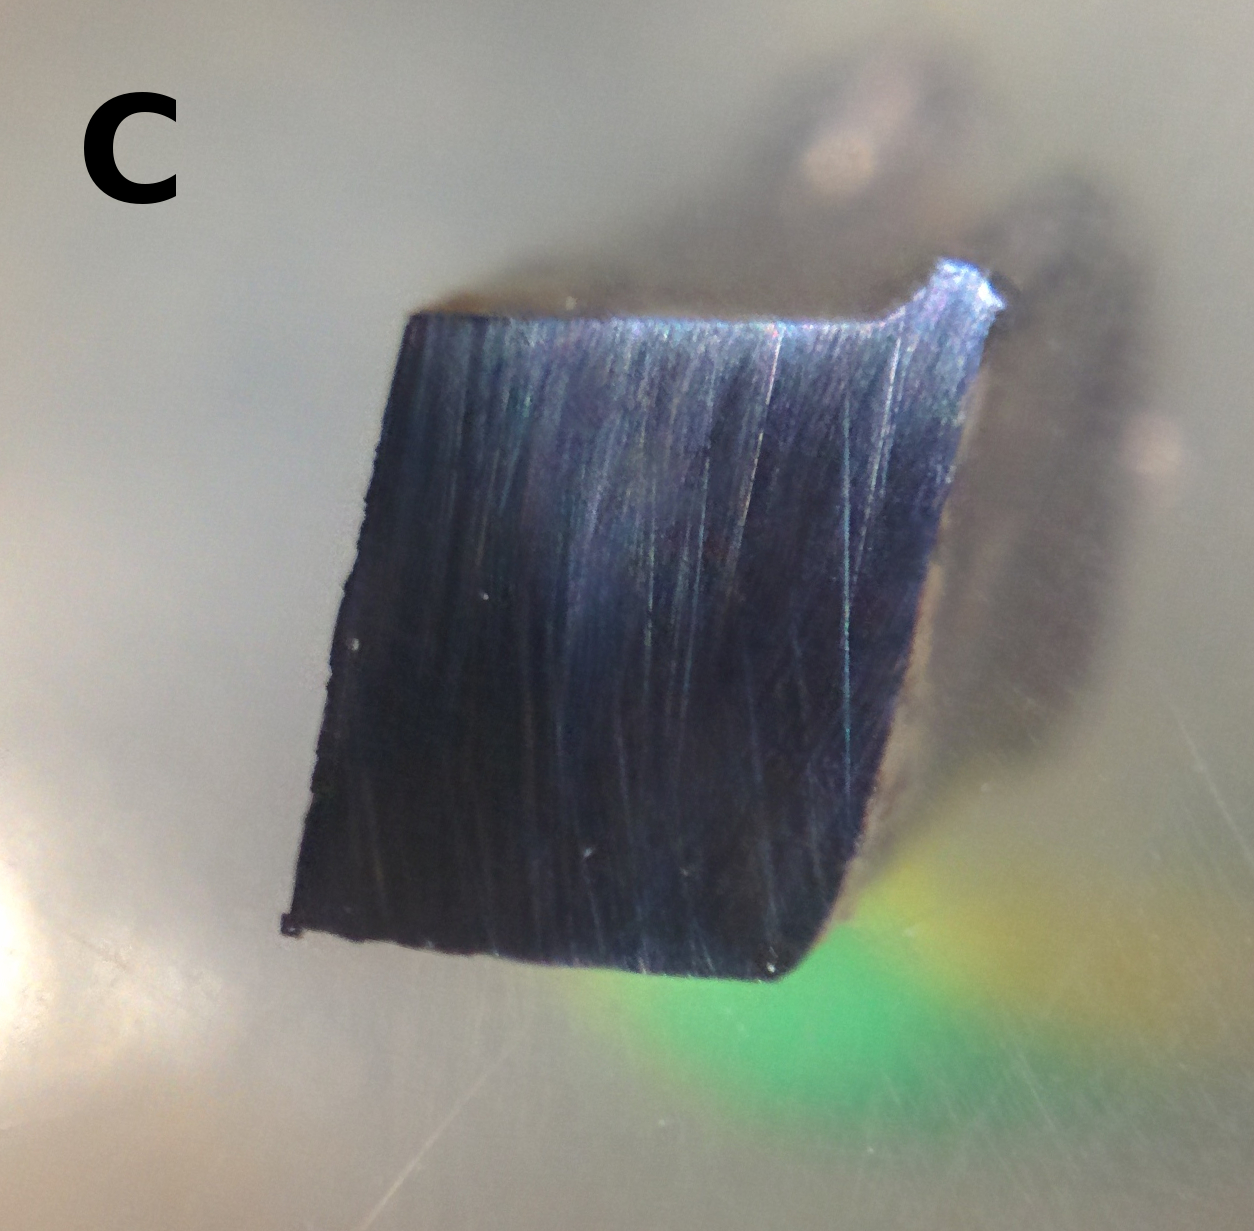
\includegraphics[width=0.24\textwidth]{cs_cut.jpg}

%\caption[Raw, and deconvoluted SECM image and microphoto of a corroding carbon-steel sample polarized anodically.]{Raw (A), and deconvoluted (B) SECM image and microphoto (C) of a corroding carbon-steel sample polarized anodically with a current density of 10 $mA/cm^2$. Measuring electrode was an antimony pH microelectrode. Potential was measured against an Ag/AgCl/3M KCl. Recorded $h$ = 100 $\upmu$m above the surface with probe movement speed of 1000 $\upmu$m/s, equilibration interval 0.4 s.}
\end{figure}
\end{frame}

\begin{frame}[plain]
\centering
The effect of electric field on potentiometric SECM imaging.
\end{frame}

\begin{frame}
\begin{center}
\frametitle{The electric field during galvanic corrosion}
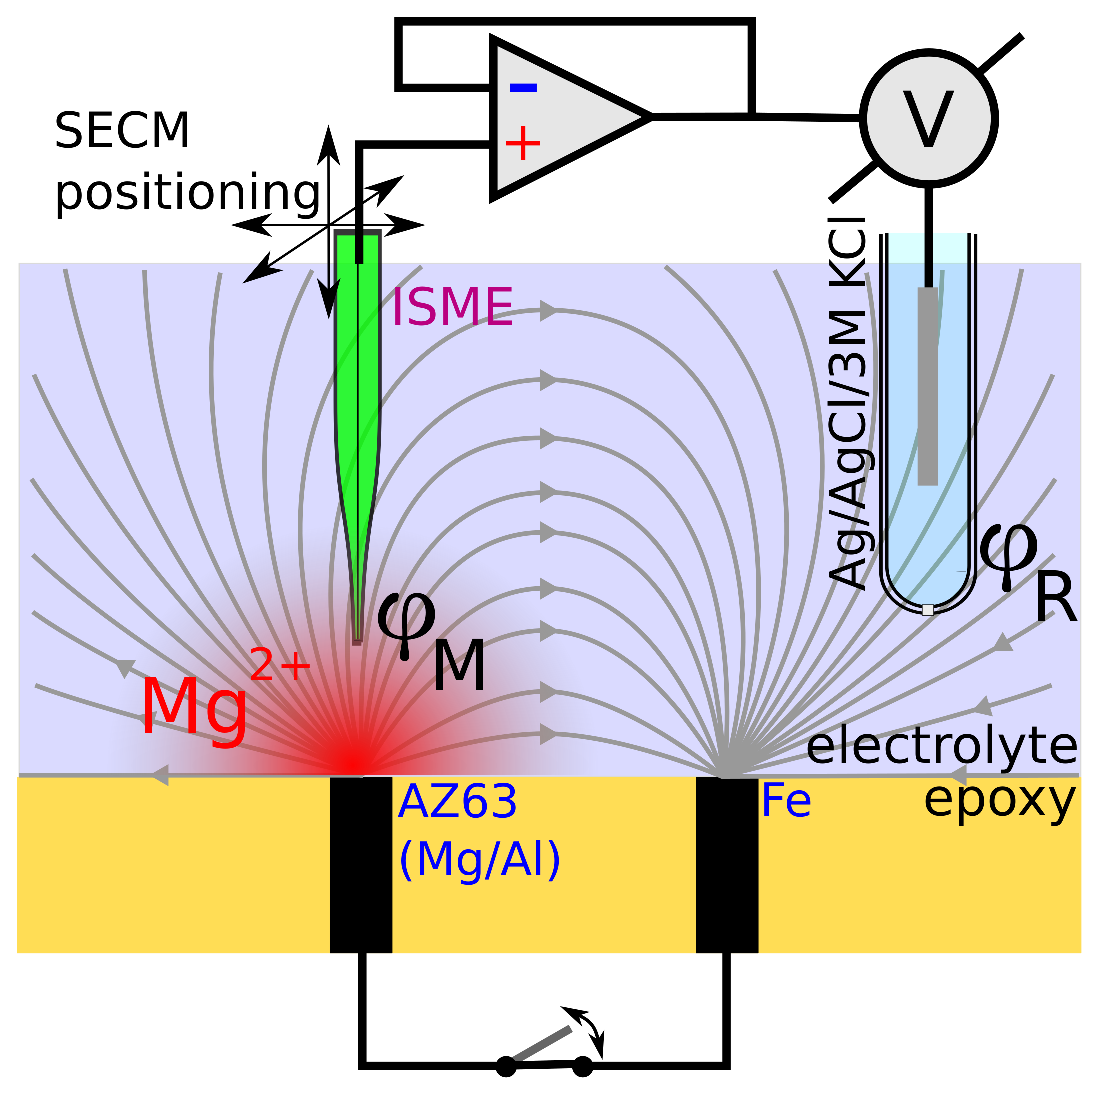
\includegraphics[width=0.5\textwidth]{field.eps}

\begin{equation*}
\Delta E=E_M-E_R + (\phi_M - \phi_R)
\label{eq:potential}
\end{equation*}
\end{center}
\end{frame}

\begin{frame}
\frametitle{The effect of electric field on the measured potential}
\framesubtitle{}
\centering
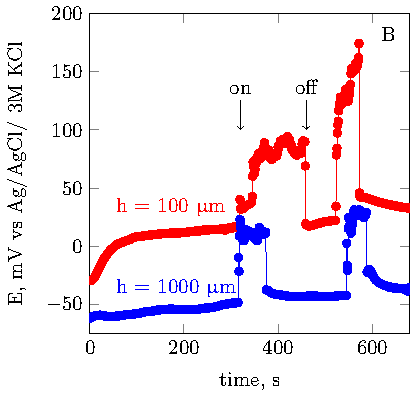
\includegraphics[width=0.466\textwidth]{field-figure1.pdf}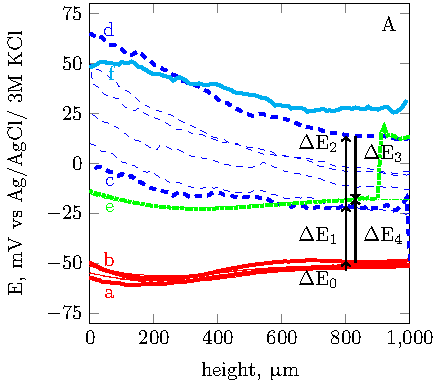
\includegraphics[width=0.5\textwidth]{field-figure0.pdf}
\end{frame}

\begin{frame}
\frametitle{The effect of electric field on potentiometric SECM imaging}
\centering
\includegraphics[trim = 10mm 20mm 0mm 10mm, clip, width=0.36\textwidth, angle=-90]{17012501.eps}\includegraphics[trim = 10mm 20mm 0mm 10mm, clip, width=0.36\textwidth, angle=-90]{17012503_deconvoluted.eps}
\end{frame}

%\begin{frame}
%\frametitle{Conclusion}
%\centering
%I have succesfully improved the potentiometric SECM.
%\end{frame}

\begin{frame}
\frametitle{Thesis 1--4}
\scriptsize
\begin{enumerate}
\item \textbf{I have shown the improved quality of potentiometric SECM images recorded with low resistance, solid-contact magnesium ion-selective microelectrodes.}
I've compared them to conventional, liquid contact microelectrodes by basic characterization and model system study to prove the improved performance.

\item \textbf{Taking advantage of the new solid-contact microelectrodes, I have studied the galvanic corrosion of magnesium} and the AZ63 magnesium alloy by mapping the concentration of dissolving ions.
The new solid contact ion selective microelectrodes allowed faster scan rates.

\item \textbf{I have estimated the corrosion current based on the SECM measurements, and compared the result with the direct measurement of corrosion current.}
After applying Faraday's Law of Electrolysis, the two results could be compared.
\textbf{They were very similar}, suggesting the applicability of SECM in obtaining quantitative results.

\item \textbf{I have designed new scanning patterns and algorithms, optimized to radially symmetric targets.}
I've proven that with these new patterns and algorithms, image distortion is lower compared to the conventional ones, by numerical simulations and experimental SECM scans.
\end{enumerate}
\end{frame}

\begin{frame}
\frametitle{Thesis 5--8}
\scriptsize
\begin{enumerate}
\setcounter{enumi}{4}
\item \textbf{I am the first who used deconvolution to reduce distortion in potentiometric SECM images.}
To prove the validity of the technique, I have compared deconvoluted images to equilibrium images scanned at a rate which allowed to record equilibrium potentials.

\item \textbf{I have successfully used deconvolution to restore potentiometric SECM images about a corroding carbon steel sample.}
Evaluation of this data was possible, because scanning time \emph{and} distortion was reduced at the same time.

\item \textbf{I have shown the possibility of blind deconvolution.}
This method can be used on measurements where the convolution function cannot be determined.

\item \textbf{I have successfully resolved the observed discrepancy in recent papers about impossibly high ion activities.}
The electric field present in many studied systems -- galvanically corroding ones in particular -- has a direct influence on the measured potential.
I have shown how big of an error can it cause.
In the system I have studied, the error was almost four orders of magnitude.
By taking this effect into account, a more accurate conclusion can be drawn.
\end{enumerate}
\end{frame}


\begin{frame}
\frametitle{List of publications}
\framesubtitle{Related to the dissertation}
\tiny
\begin{enumerate}
\item Ricardo M. Souto, \textbf{András Kiss}, Javier Izquierdo, Lívia Nagy, István Bitter, Géza Nagy, Spatially-resolved imaging of concentration distributions on corroding mag\-ne\-si\-um-based materials exposed to aqueous environments by SECM, \emph{Electrochemistry Communications 26 (2013): 25-28.}, IF.: 4.85, cited by: 31

\item \textbf{András Kiss}, Ricardo M. Souto, Géza Nagy, Investigation of Mg/Al alloy sacrificial anode corrosion with Scanning Electrochemical Microscopy, \emph{Periodica Polytechnica Chemical Engineering 57, no. 1-2 (2013): 11-14.}, IF.: 0.30, cited by: 5

\item Javier Izquierdo, \textbf{András Kiss}, Juan José Santana, Lívia Nagy, István Bitter, Hugh S. Isaacs, Géza Nagy, Ricardo M. Souto, Development of Mg$^{2+}$ ion-selective microelectrodes for potentiometric scanning electrochemical microscopy monitoring of galvanic corrosion processes, \emph{Journal of The Electrochemical Society 160, no. 9 (2013): C451-C459.}, IF.: 3.27, cited by: 23

\item \textbf{András Kiss}, Géza Nagy, New SECM scanning algorithms for improved potentiometric imaging of circularly symmetric targets, \emph{Electrochimica Acta 119 (2014): 169-174.}, IF.: 4.50, cited by: 8

\item \textbf{András Kiss}, Géza Nagy, Deconvolution of potentiometric SECM images recorded with high scan rate, \emph{Electrochimica Acta 163 (2015): 303-309.}, IF.: 4.50, cited by: 7

\item \textbf{András Kiss}, Géza Nagy, Deconvolution in potentiometric SECM, \emph{Electroanalysis 27, no. 3 (2015): 587-590.}, IF.: 2.14, cited by: 2

\item \textbf{András Kiss}, Dániel Filotás, Ricardo M Souto, Géza Nagy, The effect of electric field on potentiometric Scanning Electrochemical Microscopic imaging, \emph{Electrochemistry Communications 77 (2017): 138-141.}, IF.: 4.569
\end{enumerate}
\end{frame}

\begin{frame}
\frametitle{List of publications}
\framesubtitle{Unrelated to the dissertation}
\tiny
\begin{enumerate}
\setcounter{enumi}{7}
\item \textbf{András Kiss}, László Kiss, Barna Kovács, Géza Nagy, Air Gap Microcell for Scanning Electrochemical Microscopic Imaging of Carbon Dioxide Output. Model Calculation and Gas Phase SECM Measurements for Estimation of Carbon Dioxide Producing Activity of Microbial Sources, \emph{Electroanalysis 23, no. 10 (2011): 2320-2326.}, IF.: 2.14, cited by: 3

\item Ricardo M. Souto, Javier Izquierdo, Juan José Santana, \textbf{András Kiss}, Lívia Nagy, Géza Nagy. Progress in scanning electrochemical microscopy by coupling potentiometric and amperometric measurement modes, \emph{Current Microscopy Contributions to Advances in Science and Technology, Formatex Research Center, Badajoz (2012): 1407-1415}, cited by: 3

\item Lívia Nagy, Gergely Gyetvai, \textbf{András Kiss}, Ricardo Souto, Javier Izquierdo, Géza Nagy, Speciális célra szolgáló mikroelektródok kifejlesztése és alkalmazása, \emph{Magyar Kémiai Folyóirat 119, 2-3. (2013): 104-109.}

\item Zsuzsanna \H{O}ri, \textbf{András Kiss}, Anton Alexandru Ciucu, Constantin Mihailciuc, Cristian Dragos Stefanescu, Lívia Nagy, Géza Nagy, Sensitivity enhancement of a ,,bananatrode'' biosensor for dopamine based on SECM studies inside its reaction layer, \emph{Sensors and Actuators B: Chemical 190 (2014): 149-156.}, IF.: 4.10, cited by: 4

\item Javier Izquierdo, Bibiana M Fernández-Pérez, Dániel Filotás, Zsuzsanna Őri, \textbf{András Kiss}, Romen T Martín-Gómez, Lívia Nagy, Géza Nagy, Ricardo M Souto, Imaging of Concentration Distributions and Hydrogen Evolution on Corroding Magnesium Exposed to Aqueous Environments Using Scanning Electrochemical Microscopy, \emph{Electroanalysis 28, (2016): 2354-2366.}, IF.: 2.471, cited by: 2

\item A. El Jaouhari,  Dániel Filotás, \textbf{András Kiss}, M. Laabd, E. A. Bazzaoui, Lívia Nagy, Géza Nagy, A. Albourine, J. I. Martins, R. Wang, SECM investigation of electrochemically synthesized polypyrrole from aqueous medium, \emph{Journal of Applied Electrochemistry 46 (2016): 1199-1209.}, IF.: 2.223
\end{enumerate}
\end{frame}


\begin{frame}
\frametitle{Acknowledgements}
\scriptsize
I wish to express my sincere gratitude to \textbf{professor Dr. Géza Nagy} for introducing me to the fascinating field of electrochemistry, and for the continuous support and guidance during the work.

\vspace{4mm}

I am truly grateful to \textbf{Dr. Barna Kovács} for the enlighting discussions about microelectrode electronics. and to \textbf{Dr. Lívia Nagy} for the help received during the years of my PhD studies. I am also thankful to \textbf{Dr. Sándor Kunsági-Máté} for the support.

\vspace{4mm}

I am thankful to \textbf{Dr. Lajos Höfler} and \textbf{Dr. Balázs Csóka} for reviewing my dissertation draft. I am also thankful to all the anonymous referees who gave meaningful feedback about my work as part of the peer review process.

\vspace{4mm}

I am thankful to Professor Johan Bobacka, Ricardo M. Souto, Frank-Michael Matysik, Petr Skládal and Mohammed Bazzaoui for welcoming me in their laboratories.

\vspace{4mm}

Many thanks are due to all my colleagues and friends with whom I have worked during my years as an undergraduate and doctoral student.

\end{frame}

\begin{frame}
\centering
Thank you for your attention.
\end{frame}


\begin{frame}
	\frametitle{}
	\centering
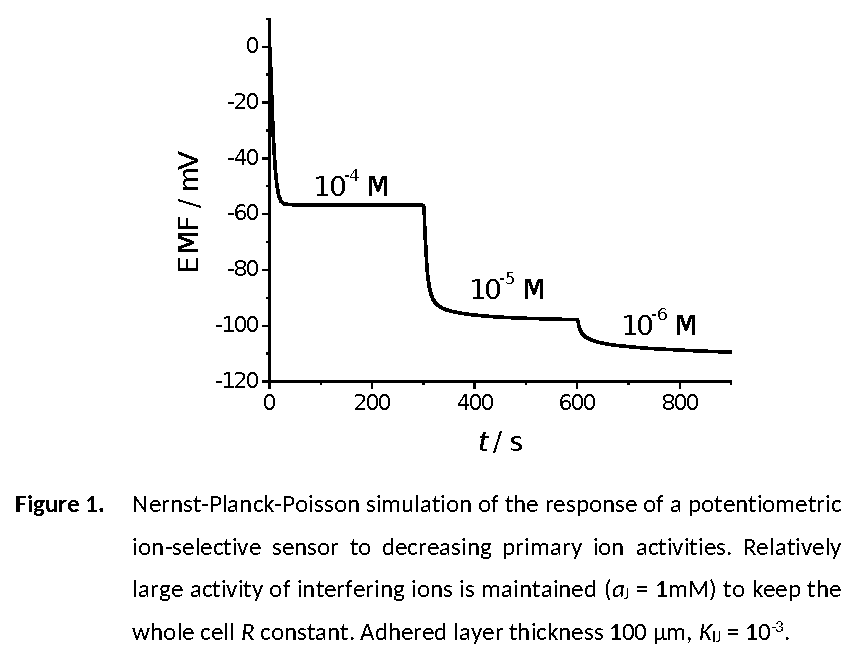
\includegraphics[width=0.8\textwidth]{HL1.eps}
\end{frame}

\begin{frame}
%	\frametitle{Calibration o}
	\centering
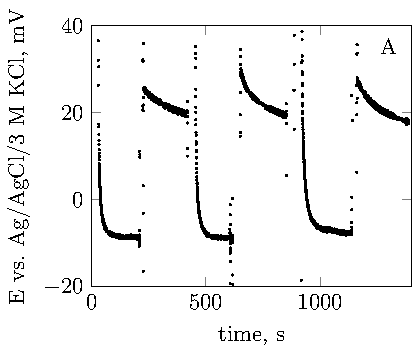
\includegraphics[width=0.45\textwidth]{phd-figure10.pdf}\hfill 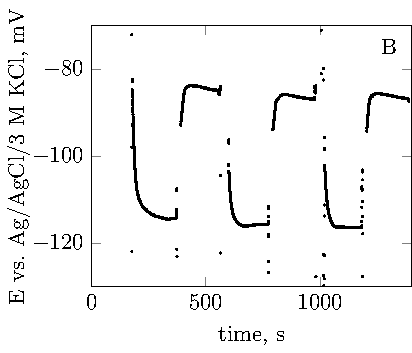
\includegraphics[width=0.45\textwidth]{phd-figure11.pdf}

\vfill

Dynamic response curves obtained for response time measurements to changes in MgCl$_2$ concentrations of 10$^{-1}$ M and 10$^{-2}$ M, in 10$^{-3}$ M NaCl.
(A) liquid-contact, and (B) solid-contact Mg$^{2+}$ ISME.
\end{frame}

\begin{frame}
\centering
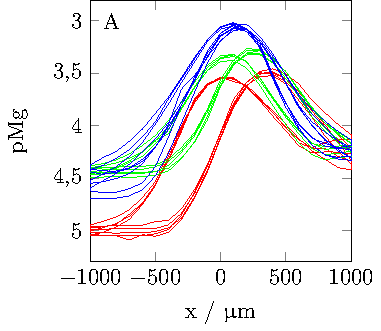
\includegraphics[width=0.45\textwidth]{phd-figure22.pdf}\hfill 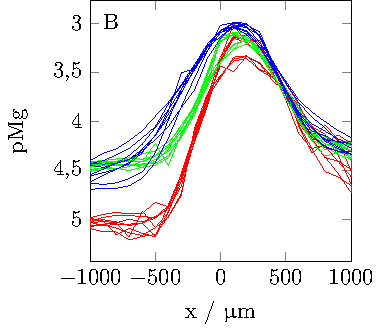
\includegraphics[width=0.45\textwidth]{phd-figure23.pdf}

\vfill

(A) Raw scan lines recorded $h$ = 100 $\upmu$m over the center of the pipette orifice, which served as a Mg$^{2+}$ ion diffusion source.
(B) Scan lines obtained after deconvolution.
$t_e$ equilibration intervals were 4.9 s (blue), 1.9 s (green), and 0.4 s (red).
Probe movement speed was 1000 $\upmu$m/s, and probe movement interval was 0.1 s.
8 scan lines were recorded in each case, 4 forward, 4 reverse scans.
\end{frame}

\begin{frame}
\centering
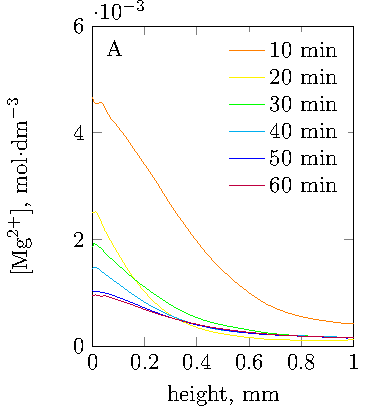
\includegraphics[width=0.25\textwidth]{phd-figure14.pdf} \includegraphics[width=0.25\textwidth]{phd-figure15.pdf}

\includegraphics[width=0.5\textwidth]{phd-figure16.pdf}
\vfill
\small
(A, B) Retracting and (C) lateral SECM linescans above the AZ63 magnesium-aluminium-zinc alloy sample initiated at different instances in time.
The AZ63 sample first was corroding spontaneously (A), then galvanically coupled to the iron sample (B). Lateral scans in (C) were recorded above the uncoupled AZ63 sample.
Scan rate: 10 $\upmu$m/s.
\end{frame}

\begin{frame}
\centering
\includegraphics[width=0.3\textwidth]{hanging.jpg}

\includegraphics[width=0.7\textwidth]{phd-figure17.pdf}

\vfill
\small
Transient response of the antimony microelectrode to analyte activity step.
The measuring and reference electrodes were dipped into buffer solutions with pH = 4 before the measurements started, and pH = 6 at t = 0 s, respectively.
Eq. 4.2 was fitted (red line) on the measurement (gray marks) from the pH step to the end of the curve when potential reaches equilibrium in the pH = 6 buffer.
\end{frame}

\begin{frame}
\centering
\includegraphics[trim = 10mm 30mm 0mm 10mm, clip, width=0.3\textwidth, angle=-90]{14103106.eps}\includegraphics[trim = 10mm 30mm 0mm 10mm, clip, width=0.3\textwidth, angle=-90]{14103106_deconvoluted.eps}%\includegraphics[trim = 20mm 30mm 0mm 20mm, clip, width=0.3\textwidth, angle=-90]{13121313_diff.eps}

\includegraphics[trim = 10mm 30mm 0mm 10mm, clip, width=0.3\textwidth, angle=-90]{14103107.eps}\includegraphics[trim = 10mm 30mm 0mm 10mm, clip, width=0.3\textwidth, angle=-90]{14103107_deconvoluted.eps}

SECM images before (A-B) and after (C-D) deconvolution.
Images recorded with the (A) meander algorithm and (B) fast comb algorithm.
Scans conducted with solid contact K$^+$ ion-selective micropipette.
\end{frame}

\begin{frame}
\begin{center}
\includegraphics[width=0.7\textwidth]{field.eps}
\end{center}
\end{frame}

\begin{frame}
\centering
\includegraphics[width=0.45\textwidth]{phd-figure20.pdf}\hfill \includegraphics[width=0.45\textwidth]{phd-figure21.pdf}
\vfill
(A) Raw, and, (B) deconvoluted SECM linescans above the center of the target, at h = 100 $\upmu$m height, using three different equilibration periods: 0.5 s, (green), 1 s, (blue), and 5 s, (red).
\end{frame}

\end{document}
